\documentclass[11pt]{article}

% ── Packages ──────────────────────────────────────────────────
\usepackage[utf8]{inputenc}
\usepackage[T1]{fontenc}
\usepackage{lmodern}
\usepackage[margin=1in]{geometry}
\usepackage{amsmath,amssymb,amsfonts}
\usepackage{booktabs}
\usepackage{graphicx}
\usepackage[hidelinks]{hyperref}
\usepackage{xcolor}
\usepackage{caption}
\usepackage{subcaption}
\usepackage{multirow}
\usepackage{array}
\usepackage{tabularx}
\usepackage{float}
\usepackage{placeins}
\usepackage{enumitem}
\usepackage{microtype}
\usepackage{authblk}
\usepackage{natbib}
\bibliographystyle{plainnat}
\graphicspath{{figures/}{../output/figures/}{../output/mitigations/figures/}}

% ── Custom commands ───────────────────────────────────────────
\newcommand{\ie}{i.e.,\ }
\newcommand{\eg}{e.g.,\ }
\newcommand{\cf}{cf.\ }
\newcommand{\etal}{et~al.}
\newcommand{\wrt}{w.r.t.\ }
\newcommand{\pval}[1]{$p #1$}

% ── Title ─────────────────────────────────────────────────────
\title{\textbf{No One Gets an A: Distributional Bias in LLM Text Scoring}}

\author{Idrees Aziz}
\author{Mahir Sadikhov}
\affil{Independent Researchers}

\date{}

\begin{document}
\maketitle

% ══════════════════════════════════════════════════════════════
% ABSTRACT
% ══════════════════════════════════════════════════════════════
\begin{abstract}
When large language models (LLMs) are asked to rate text quality on a numeric scale, they systematically avoid extreme scores---compressing their responses into a narrow interior band regardless of true quality variation. We present a controlled experiment measuring this \emph{score compression} effect across eleven language models spanning 3.8B to 228B parameters, using 9{,}000 text samples derived from 150 expert-authored articles sourced from The Conversation (theconversation.com). Each article is degraded along four independent quality axes (grammar, coherence, information, lexical sophistication) at five controlled intensity levels, producing a known ground-truth quality gradient. In a detailed two-model study of GPT-5~mini and Gemini~3~Flash, neither model ever assigns a score of 0 or 10 on a 0--10 scale---and the same boundary avoidance holds for four additional models---despite calibrated simulations predicting hundreds of such scores. Both compress the effective scoring range to approximately 62--69\% of the ideal range, with compression statistically confirmed via block-bootstrap confidence intervals. A three-way linear mixed-effects model reveals significant main effects of degradation level, axis, and model, along with all two- and three-way interactions. Extending to nine additional models, we find compression ratios ranging from 0.02 (Mistral~7B) to 0.69 (GPT-5~mini), with a positive correlation between model size and compression ratio (Pearson $r = 0.78$, $p = 0.012$). Across all eleven models and approximately 99{,}000 total evaluations, score compression is universal. We evaluate five mitigation strategies: quantile normalization, expected-score rescaling, auxiliary regression, asymmetry correction, and contrastive anchor prompting. On a controlled nine-model comparison, auxiliary regression yields the largest gains in pairwise accuracy ($0.518 \to 0.702$) and expected-score rescaling improves rank correlation ($\rho: 0.458 \to 0.490$). Quantile normalization expands compression ratios to $>$0.92 while preserving rank order. Contrastive anchor prompting produces mixed results across two API models (Gemini: $+0.035$; GPT: $-0.110$ in $\rho$). A post-hoc affine calibration experiment on a held-out test set reduces RMSE by 12--27\%, confirming that the distortion is systematic and partially correctable. These findings demonstrate that LLM-based text evaluation is subject to a robust distributional bias---confirmed across approximately 99{,}000 evaluations spanning eleven models---with practical implications for any application relying on LLM-generated quality ratings.
\end{abstract}

\textbf{Keywords:} large language models, text evaluation, score compression, distributional bias, calibration, mitigation

% ══════════════════════════════════════════════════════════════
% 1. INTRODUCTION
% ══════════════════════════════════════════════════════════════
\section{Introduction}
\label{sec:intro}

Large language models are increasingly deployed as automated text evaluators---grading student essays, rating content quality, scoring summaries, and benchmarking generated text~\citep{zheng2023judging}. These applications implicitly assume that LLMs can map text quality onto numeric scales with reasonable fidelity. Yet anecdotal and preliminary evidence suggests that LLMs exhibit a systematic reluctance to use the extremes of any provided rating scale. A pristine, publication-quality text that a human expert might comfortably rate 9 or 10 out of 10 consistently receives a 7 or 8 from an LLM. Conversely, heavily corrupted, barely readable text rarely drops below 2 or 3.

This behavior---which we term \emph{score compression}---has significant practical consequences. If the effective scoring range is compressed from $[0, 10]$ to approximately $[2, 9]$, then the discriminative resolution of the scale is reduced by 30\% or more. Fine-grained quality distinctions are lost, ranking reliability degrades, and threshold-based decisions (\eg ``pass if score $\geq 7$'') become miscalibrated.

To quantify this gap precisely: under a naive linear calibration model, a text degraded to fraction $\lambda$ of its original quality should receive a score $S = 10(1 - \lambda)$. Instead, we observe approximately $S \approx 8 - 6.5\lambda$ for GPT-5~mini and $S \approx 8 - 6.2\lambda$ for Gemini~3~Flash---the intercept falls short of~10 and the slope attains only $\sim$65\% of the ideal gradient, compressing the usable scoring range by roughly a third.

In this paper, we present a rigorous, controlled experiment designed to measure score compression precisely. Our approach has three key features:

\begin{enumerate}[nosep]
    \item \textbf{Known ground-truth quality gradient.} We start from texts of verified high quality (expert-authored articles from The Conversation) and apply mathematically defined degradations at controlled intensity levels, producing a continuous quality spectrum from pristine to severely corrupted.
    \item \textbf{Axis isolation.} Degradation is applied along four independent axes---grammar, coherence, information content, and lexical sophistication---allowing us to assess whether compression varies by quality dimension.
    \item \textbf{Multi-model comparison.} We evaluate two frontier models in depth (GPT-5~mini from OpenAI and Gemini~3~Flash from Google) and extend the analysis to nine additional models spanning 3.8B to 228B parameters---including open-weight models from Meta, Google, Microsoft, Alibaba, Mistral~AI, and MiniMax---to assess how compression varies with model scale and architecture.
\end{enumerate}

We declare three primary outcomes \emph{a priori}:
\begin{enumerate}[nosep]
    \item The compression ratio (observed scoring range divided by ideal range) per model.
    \item The average linear regression slope of score on degradation level, per model.
    \item The median paired score difference between models on identical samples.
\end{enumerate}

Our contributions go beyond documenting central tendency bias in a new modality. While prior work has noted qualitatively that LLMs tend toward ``safe'' interior scores, we provide: (i)~a \emph{quantified} compression magnitude against an algebraically defined ground truth, (ii)~cross-model replication across eleven models showing the effect generalizes across providers, architectures, and scales, (iii)~axis-specific sensitivity profiles revealing that compression severity depends on the quality dimension under evaluation, (iv)~a calibration recovery experiment demonstrating that a simple affine transform reduces the calibration gap by 12--27\%, and (v)~a systematic evaluation of five mitigation strategies---quantile normalization, expected-score rescaling, auxiliary regression, asymmetry correction, and contrastive anchor prompting---showing that post-hoc corrections can partially recover lost discriminative range.

% ══════════════════════════════════════════════════════════════
% 2. RELATED WORK
% ══════════════════════════════════════════════════════════════
\section{Related Work}
\label{sec:related}

The use of LLMs as evaluators has grown rapidly since the introduction of ``LLM-as-a-judge'' frameworks~\citep{zheng2023judging}. Studies have examined positional bias (preference for responses presented first or second), verbosity bias (preference for longer outputs), and self-enhancement bias (preference for outputs from the same model family)~\citep{wang2023large}. However, the distributional properties of LLM-generated numeric scores---particularly the systematic avoidance of scale endpoints---have received comparatively little attention.

\textbf{Central tendency bias in human rating.} Central tendency bias is well-documented in psychometrics: human raters systematically avoid extreme categories on Likert and other bounded scales, producing distributions compressed around the midpoint~\citep{stevens1971issues}. This tendency is modulated by rater expertise, scale length, and anchoring~\citep{guilford1954psychometric}. In automated essay scoring (AES), neural models trained on human ratings inherit these distributional properties, and various calibration and normalization methods have been explored to recover lost range~\citep{ke2019automated}. Whether LLMs exhibit analogous biases due to their training on human-generated rating data, reinforcement learning from human feedback (RLHF), or architectural constraints remains an open question.

\textbf{LLM-based evaluation.} Recent work has increasingly employed LLMs as stand-in evaluators for machine translation~\citep{kocmi2023large}, summarization, and open-ended generation. \citet{kocmi2023large} showed that GPT-based metrics achieve state-of-the-art correlation with human MT judgments but did not examine the distributional properties of the scores themselves. \citet{liu2023geval} demonstrated that LLM-generated evaluation scores exhibit significant miscalibration and proposed decomposed prompting strategies to improve alignment with human judgments.

Our work differs from these studies in that we do not compare LLM judgments against human judgments on naturalistic text. Instead, we construct a synthetic but precisely controlled quality gradient, enabling direct measurement of calibration fidelity without human annotation noise.

% ══════════════════════════════════════════════════════════════
% 3. EXPERIMENTAL DESIGN
% ══════════════════════════════════════════════════════════════
\section{Experimental Design}
\label{sec:design}

\subsection{Corpus Construction}

The corpus consists of 150 articles sourced from The Conversation (theconversation.com)---a media platform where academic experts and researchers write evidence-based articles for a general audience. Each article undergoes professional editorial review before publication, including copy-editing and fact-checking by staff editors, representing a consistently high standard of expository prose. Articles are drawn from five broad categories (Arts \& Culture, Business \& Economy, Health, Politics \& Society, Science \& Technology) to ensure topical diversity. Articles are selected to maintain full-text integrity without truncation while controlling API costs.

\subsection{Degradation Engine}

Each article is degraded along exactly one of four orthogonal quality axes at one of five intensity levels $\lambda \in \{0.0, 0.2, 0.4, 0.6, 0.8\}$:

\begin{itemize}[nosep]
    \item \textbf{Grammar} ($G$): Introduces surface-level mechanical errors (keyboard typos, agreement violations, tense swaps, article errors, confusable homophones, preposition errors, word-order disruption) via a nine-stage pipeline.
    \item \textbf{Coherence} ($C$): Disrupts logical flow by performing bounded random swaps of sentence order, preserving all content and grammar.
    \item \textbf{Information} ($I$): Progressively deletes content through a five-phase pipeline targeting parentheticals, modifiers, prepositional phrases, subordinate clauses, and content words.
    \item \textbf{Lexical} ($L$): Flattens vocabulary diversity by replacing content words with more common synonyms using GloVe embeddings, simulating lexical simplification.
\end{itemize}

At $\lambda = 0$, the original text is returned unchanged. The maximum degradation level is $\lambda = 0.8$ rather than $1.0$: at full intensity, several axes produce output that is no longer parseable as coherent text (\eg information deletion removes nearly all content words, grammar corruption introduces errors in every sentence), which risks triggering refusal or confusion rather than meaningful scoring. Capping at $0.8$ ensures that even maximally degraded texts remain recognizably textual.

The goal is controlled perturbation with known ground truth, not ecological validity; the degradation axes are designed to isolate specific quality dimensions in a way that naturalistic quality variation cannot. Each degradation function is deterministic: a per-sample seed is computed via $\text{MD5}(\text{title} \| \text{axis} \| \text{level} \| \text{rep}) \bmod 2^{31}$, ensuring bitwise reproducibility.

\subsection{Factorial Design}

The full experiment follows a $150 \times 4 \times 5 \times 3$ factorial design:
\begin{equation}
    N = |\mathcal{C}| \times |\mathcal{A}| \times |\mathcal{L}| \times R = 150 \times 4 \times 5 \times 3 = 9{,}000
    \label{eq:design}
\end{equation}

\noindent where $\mathcal{C}$ is the set of corpus articles, $\mathcal{A}$ the set of degradation axes, $\mathcal{L}$ the set of intensity levels, and $R = 3$ the number of repetitions per condition, yielding 9{,}000 samples per model.

\subsection{Scoring Protocol}

Each sample is presented in isolation with a minimal prompt: the system message instructs ``Rate the quality of the following text from 0 to 10. Respond with ONLY the number.'' No rubric, examples, or reference texts are provided. This design measures the model's intrinsic calibration on an unanchored scale.

\begin{table}[t]
\centering
\caption{Models and configurations. The two primary models (GPT-5~mini, Gemini~3~Flash) are evaluated at full factorial scale (9{,}000 samples each). Nine additional models are scored on the same 9{,}000 samples for the multi-model extension.}
\label{tab:models}
\begin{tabular}{@{}llrlll@{}}
\toprule
\textbf{Model} & \textbf{Provider} & \textbf{Params} & \textbf{Access} & \textbf{Temp.} & \textbf{Logprobs} \\
\midrule
GPT-5 mini & OpenAI & --- & API & 1.0 & No \\
Gemini 3 Flash & Google & --- & API & 0.0 & No \\
\midrule
GPT-OSS 120B & Fireworks & 120B & API & 0.0 & Yes \\
MiniMax M2P1 & Fireworks & 228B & API & 0.0 & Yes \\
Gemma 2 9B & Local (Ollama) & 9B & Local & 0.0 & Yes \\
Llama 3.1 8B & Local (Ollama) & 8B & Local & 0.0 & Yes \\
Mistral 7B & Local (Ollama) & 7B & Local & 0.0 & Yes \\
Phi-4 14B & Local (Ollama) & 14B & Local & 0.0 & Yes \\
Phi-4 mini & Local (Ollama) & 3.8B & Local & 0.0 & Yes \\
Qwen 2.5 14B & Local (Ollama) & 14B & Local & 0.0 & Yes \\
Qwen 2.5 7B & Local (Ollama) & 7B & Local & 0.0 & Yes \\
\bottomrule
\end{tabular}
\end{table}

GPT-5~mini is a reasoning model that allocates internal thinking tokens before producing output; temperature cannot be set below 1.0.\footnote{OpenAI API documentation for reasoning models (o-series and derivatives) states: ``temperature is fixed at 1 and cannot be modified.'' See \url{https://platform.openai.com/docs/guides/reasoning}.} Gemini~3~Flash uses minimal thinking with temperature 0.0 for determinism. The nine extension models all use temperature 0.0 and return token-level log-probabilities, enabling logprob-based mitigation strategies (Section~\ref{sec:mitigation}).

% ══════════════════════════════════════════════════════════════
% 4. RESULTS
% ══════════════════════════════════════════════════════════════
\section{Results}
\label{sec:results}

We organize results around our three primary outcomes, followed by secondary analyses.

\subsection{Score Distributions}

Table~\ref{tab:dist} summarizes the overall score distributions for all eleven models. Most models use only a narrow subset of the 0--10 scale: the two primary models GPT-5~mini ($[1, 9]$) and Gemini~3~Flash ($[2, 9]$) never assign 0 or 10 across 9{,}000 samples each, nor do Gemma~2~9B, Llama~3.1~8B, Phi-4~14B, or Qwen~2.5~14B. Five models do produce occasional extreme scores, though rarely: MiniMax~M2P1 assigns 686 tens (7.7\% of samples), GPT-OSS~120B assigns 394 zeros (4.4\%), while Mistral~7B, Phi-4~mini, and Qwen~2.5~7B produce fewer than 25 extreme scores each. Score means range from 4.23 (GPT-OSS~120B) to 8.62 (Qwen~2.5~7B), with smaller models clustering at higher means and lower standard deviations---consistent with more severe score compression. Figure~\ref{fig:histograms} visualizes all eleven score distributions, with red annotations highlighting zero-count bins.

\begin{figure}[!htbp]
\centering
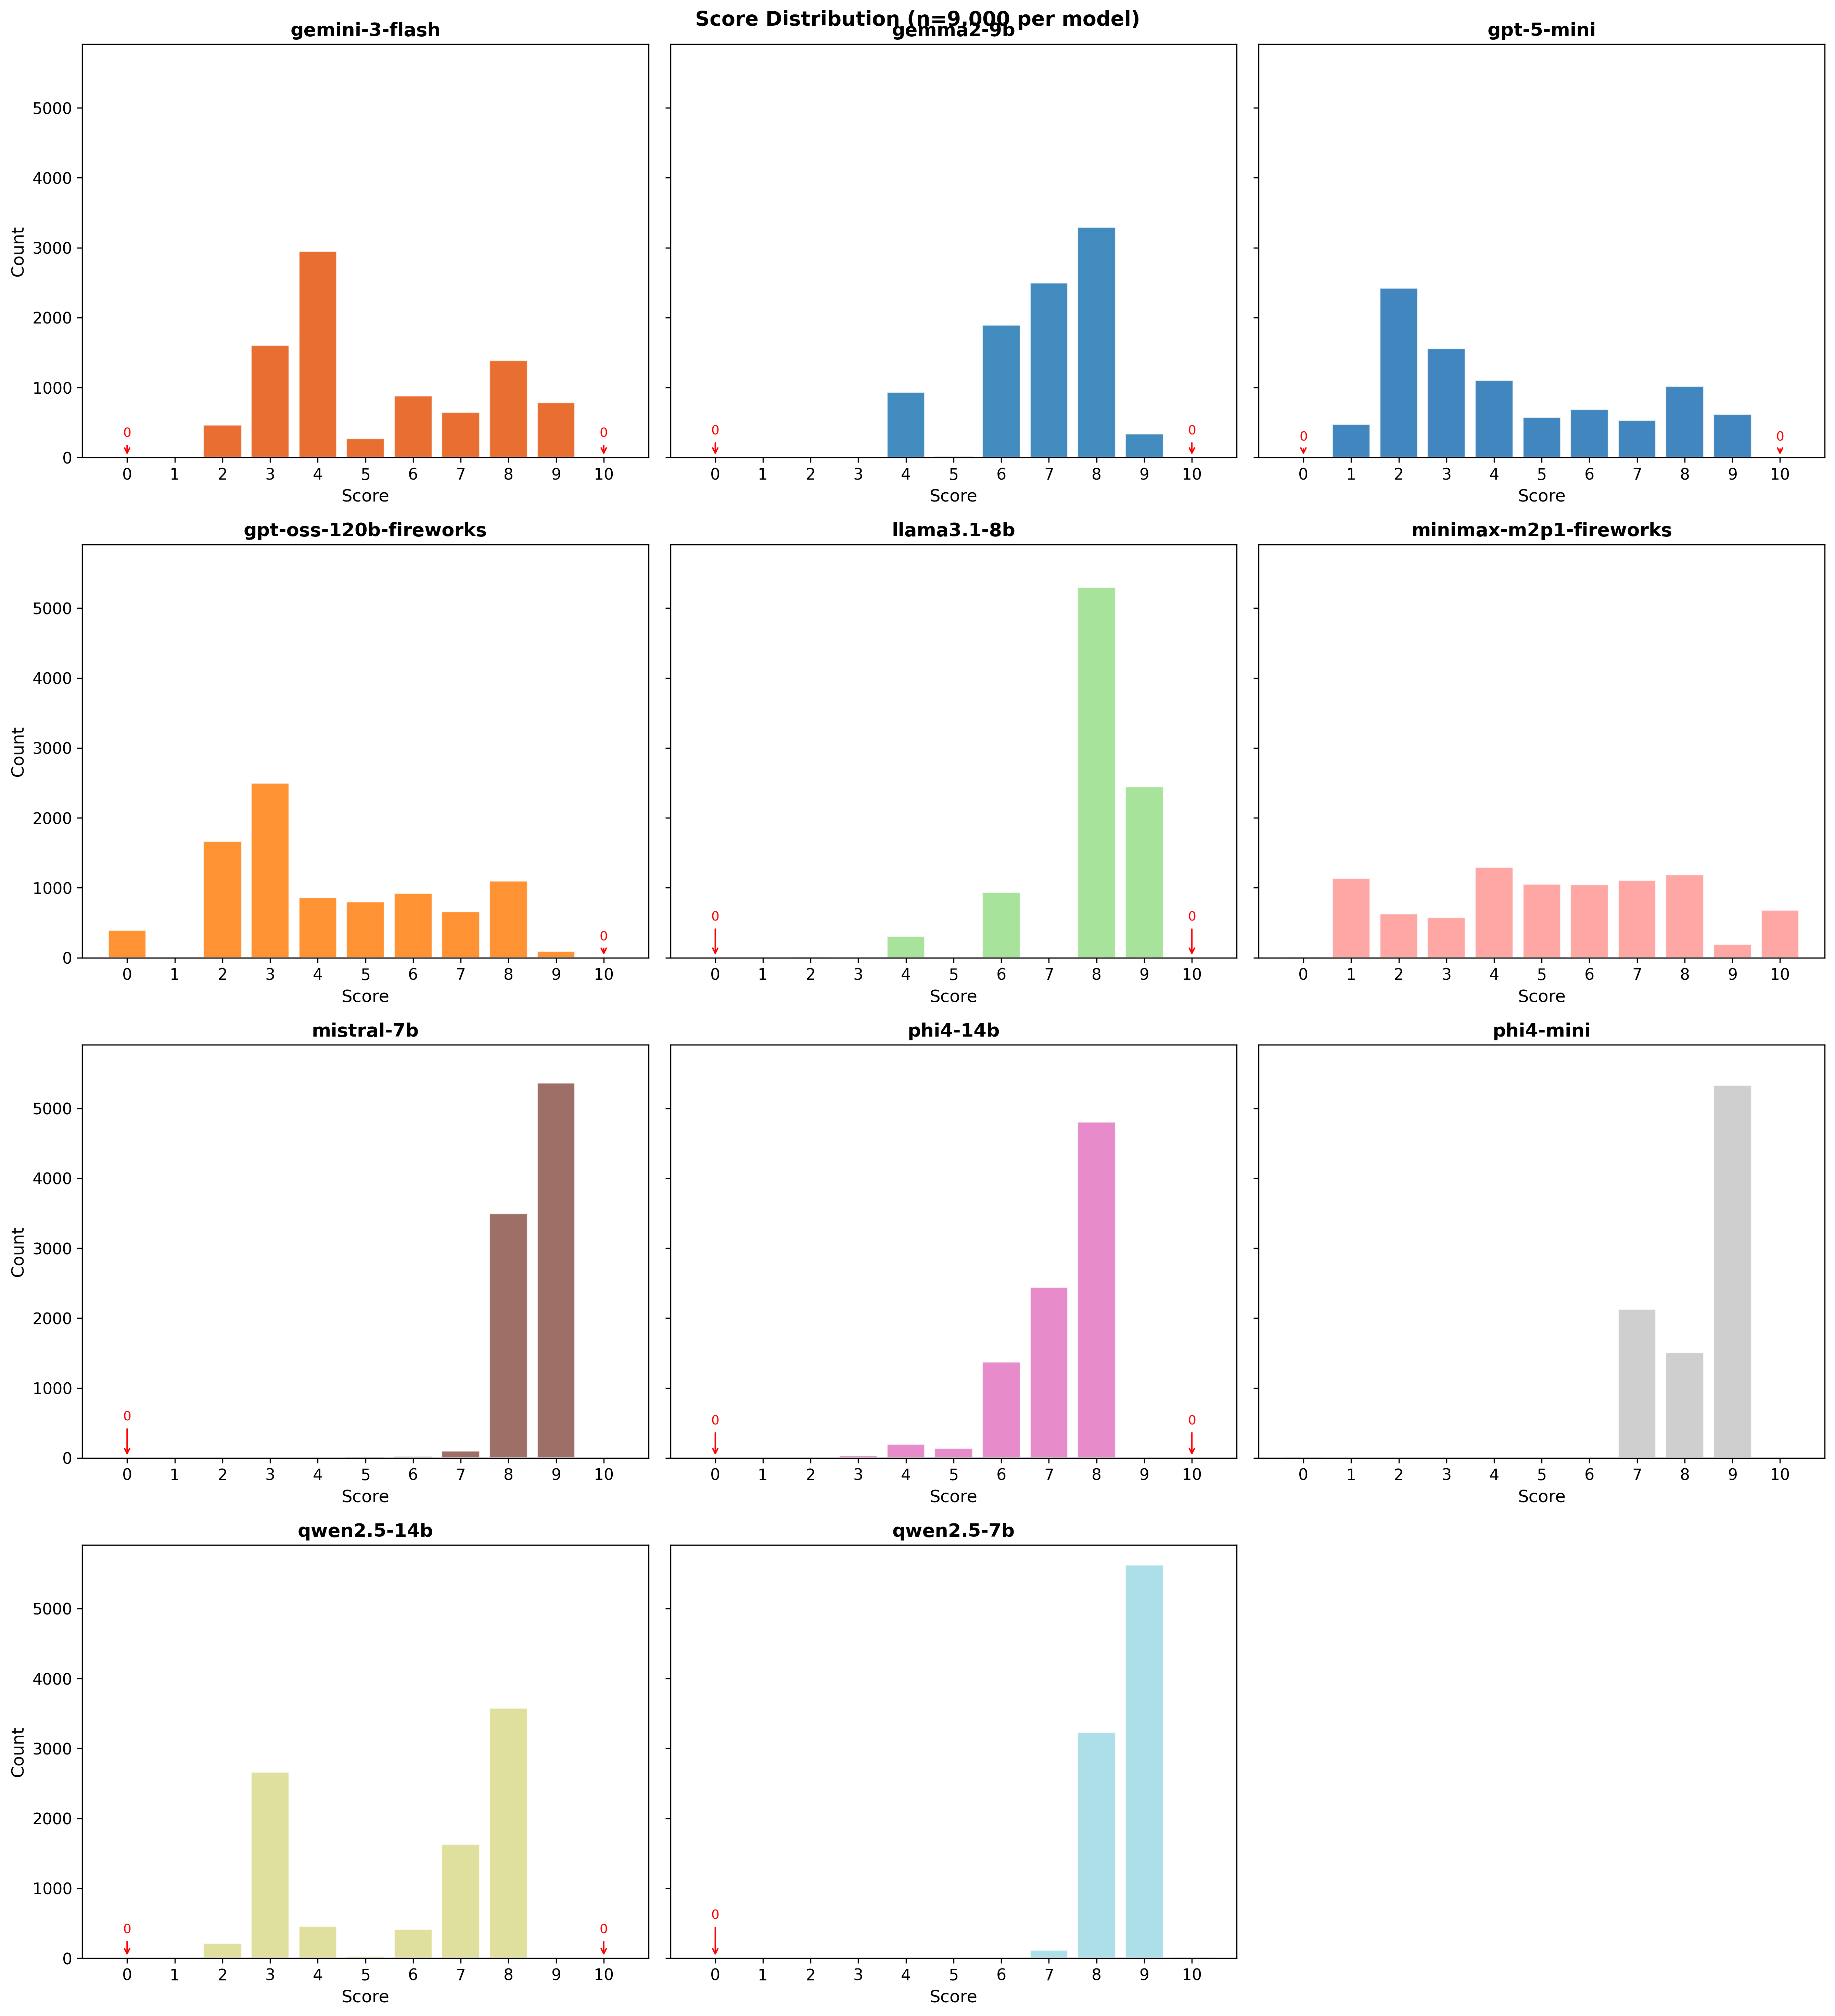
\includegraphics[width=\textwidth]{G3_score_histograms.png}
\caption{Overall score distributions for all eleven models ($n \approx 9{,}000$ per model). Red ``0'' annotations mark score bins with zero counts; bars that appear empty but lack an annotation have small but non-zero counts. Six of eleven models never assign 0 or 10; five produce rare extreme scores (see Table~\ref{tab:dist}).}
\label{fig:histograms}
\end{figure}

\begin{table}[H]
\centering
\caption{Descriptive statistics of score distributions for all eleven models, ordered by compression ratio (Table~\ref{tab:compression}). \#0s and \#10s denote the number of times a model assigned the minimum or maximum score.}
\label{tab:dist}
\small
\begin{tabular}{@{}lrccrccc@{}}
\toprule
\textbf{Model} & $n$ & \textbf{Mean} & \textbf{SD} & \textbf{Range} & \textbf{Skew} & \textbf{\#0s} & \textbf{\#10s} \\
\midrule
GPT-5 mini & 9{,}000 & 4.32 & 2.46 & 1--9 & 0.57 & 0 & 0 \\
Gemini 3 Flash & 9{,}000 & 5.21 & 2.15 & 2--9 & 0.43 & 0 & 0 \\
GPT-OSS 120B & 9{,}000 & 4.23 & 2.25 & 0--9 & 0.35 & 394 & 0 \\
Qwen 2.5 14B & 9{,}000 & 5.89 & 2.24 & 2--8 & $-$0.43 & 0 & 0 \\
MiniMax M2P1 & 8{,}933 & 5.23 & 2.67 & 0--10 & $-$0.01 & 8 & 686 \\
Gemma 2 9B & 9{,}000 & 6.91 & 1.30 & 3--9 & $-$0.91 & 0 & 0 \\
Phi-4 14B & 9{,}000 & 7.27 & 0.97 & 3--8 & $-$1.49 & 0 & 0 \\
Llama 3.1 8B & 9{,}000 & 7.92 & 1.12 & 2--9 & $-$1.85 & 0 & 0 \\
Phi-4 mini & 8{,}991 & 8.34 & 0.91 & 0--10 & $-$1.88 & 15 & 3 \\
Qwen 2.5 7B & 8{,}998 & 8.62 & 0.52 & 6--10 & $-$0.75 & 0 & 21 \\
Mistral 7B & 9{,}000 & 8.58 & 0.55 & 5--10 & $-$1.05 & 0 & 5 \\
\bottomrule
\end{tabular}
\end{table}

\begin{figure}[H]
\centering
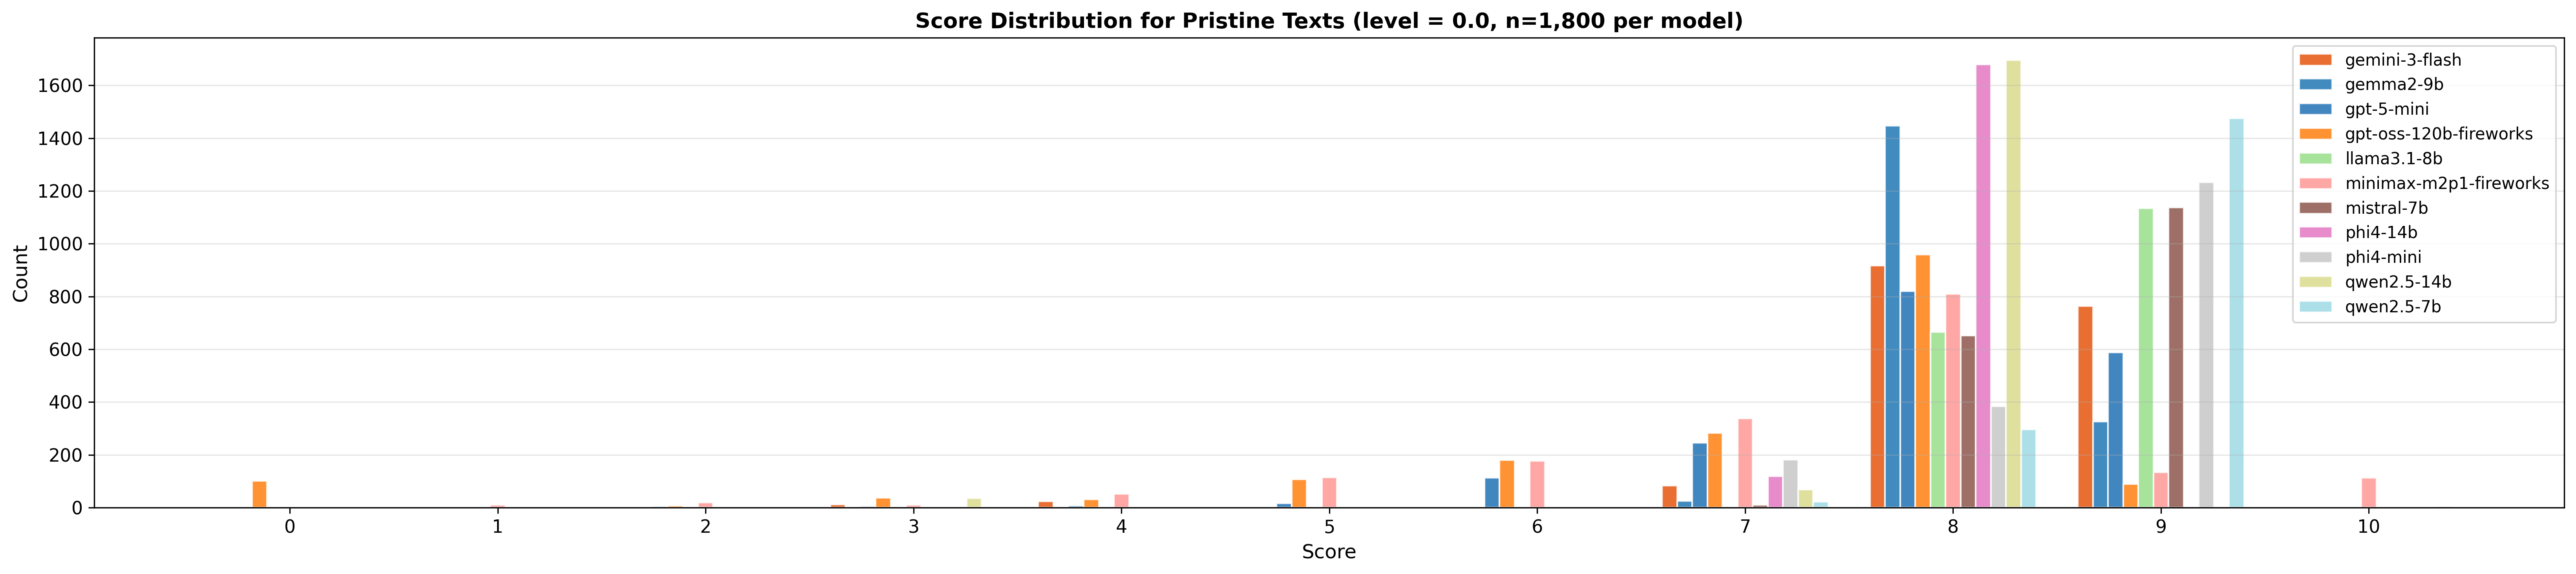
\includegraphics[width=\textwidth]{G4_undegraded_dist.png}
\caption{Score distribution for pristine (undegraded, $\lambda = 0.0$) texts only ($n = 1{,}800$ per model). All models concentrate pristine scores in a narrow range at the top of the scale, with most never assigning 10 even to expert-authored, editorially curated articles.}
\label{fig:undegraded}
\end{figure}

\subsection{Boundary Avoidance}

To assess whether the absence of extreme scores is merely a consequence of the experimental design (no fully pristine or fully destroyed texts), we compare observed boundary counts against a calibrated baseline. We fit a linear model of score on degradation level per model, simulate 100 datasets by adding Gaussian noise with the observed residual standard deviation, and count how often scores of 0 and 10 appear. For the six models that never assign 0 or 10, the simulations predict substantial counts at both boundaries: GPT-5~mini should produce $\sim$542 zeros and $\sim$122 tens; Gemini~3~Flash should produce $\sim$73 zeros and $\sim$147 tens; yet both observed counts are zero. Gemma~2~9B, Llama~3.1~8B, Phi-4~14B, and Qwen~2.5~14B show similar patterns of complete boundary avoidance despite simulated predictions of tens to hundreds of extreme scores. For the five models that do produce some extreme scores (GPT-OSS~120B, MiniMax~M2P1, Mistral~7B, Phi-4~mini, Qwen~2.5~7B), the observed counts are still far below simulation predictions (\eg Mistral produces 5 tens vs.~$\sim$407 predicted). This constitutes strong evidence of active boundary avoidance across the model landscape.

\FloatBarrier
\subsection{Primary Outcome 1: Compression Ratio}

We define the compression ratio as the observed mean score range divided by the expected range under a naive linear calibration model. This reference assumes that an ideal linear scorer would map degradation level $\lambda$ to a score $S = 10(1 - \lambda)$, yielding 10 for pristine text and linearly decreasing with degradation intensity. Under this model, the expected score span between $\lambda = 0$ and $\lambda = 0.8$ is $10(1 - 0) - 10(1 - 0.8) = 8$ points. We use this span rather than the full 0--10 range because our experiment does not include $\lambda = 1.0$ (see below), and the reference must match the experimental conditions:
\begin{equation}
    \rho = \frac{\bar{S}(\lambda = 0) - \bar{S}(\lambda = 0.8)}{10(1 - 0) - 10(1 - 0.8)} = \frac{\bar{S}(0) - \bar{S}(0.8)}{8}
    \label{eq:compression}
\end{equation}

A value of $\rho = 1$ indicates no compression (exact agreement with the naive reference); $\rho < 1$ indicates compression.

\begin{table}[!t]
\centering
\caption{Compression ratio (CR) with 95\% block-bootstrap CIs (10{,}000 iterations, resampling articles) and Spearman $\rho$ against proxy ground truth for all eleven models. All CIs exclude 1.0, confirming statistically significant compression.}
\label{tab:compression}
\small
\begin{tabular}{@{}lrccc@{}}
\toprule
\textbf{Model} & \textbf{Params} & $\hat{\rho}_{\text{CR}}$ & \textbf{95\% CI} & \textbf{Spearman} $\rho$ \\
\midrule
GPT-5 mini & --- & 0.685 & [0.667, 0.700] & 0.729 \\
Gemini 3 Flash & --- & 0.620 & [0.603, 0.635] & 0.801 \\
GPT-OSS 120B & 120B & 0.504 & [0.470, 0.537] & 0.617 \\
Qwen 2.5 14B & 14B & 0.446 & [0.431, 0.461] & 0.618 \\
MiniMax M2P1 & 228B & 0.420 & [0.392, 0.447] & 0.473 \\
Gemma 2 9B & 9B & 0.299 & [0.288, 0.311] & 0.704 \\
Phi-4 14B & 14B & 0.177 & [0.168, 0.187] & 0.548 \\
Llama 3.1 8B & 8B & 0.157 & [0.148, 0.166] & 0.464 \\
Phi-4 mini & 3.8B & 0.078 & [0.067, 0.089] & 0.239 \\
Qwen 2.5 7B & 7B & 0.056 & [0.049, 0.064] & 0.324 \\
Mistral 7B & 7B & 0.026 & [0.018, 0.034] & 0.138 \\
\bottomrule
\end{tabular}
\end{table}

All eleven models compress the effective scoring range below the ideal (Table~\ref{tab:compression}). Compression ratios vary widely, from CR $= 0.026$ (Mistral~7B, which collapses nearly all scores into a single bin) to CR $= 0.685$ (GPT-5~mini). The two primary models---GPT-5~mini (69\%) and Gemini~3~Flash (62\%)---use the most of the available range. All confidence intervals exclude 1.0, confirming that compression is statistically robust across every model tested. Smaller models tend to exhibit more extreme compression: models below 10B parameters all achieve CRs below 0.30, while models above 100B all exceed 0.42 (Section~\ref{sec:multimodel} explores this trend further). Notably, compression ratio and rank correlation are not perfectly correlated: Gemma~2~9B achieves a higher Spearman $\rho$ (0.704) than several models with higher CRs, indicating that a model can rank texts well despite compressing them into a narrow range. Figure~\ref{fig:calibration} visualizes the compression gap against the naive calibration line for the two primary models.

\begin{figure}[H]
\centering
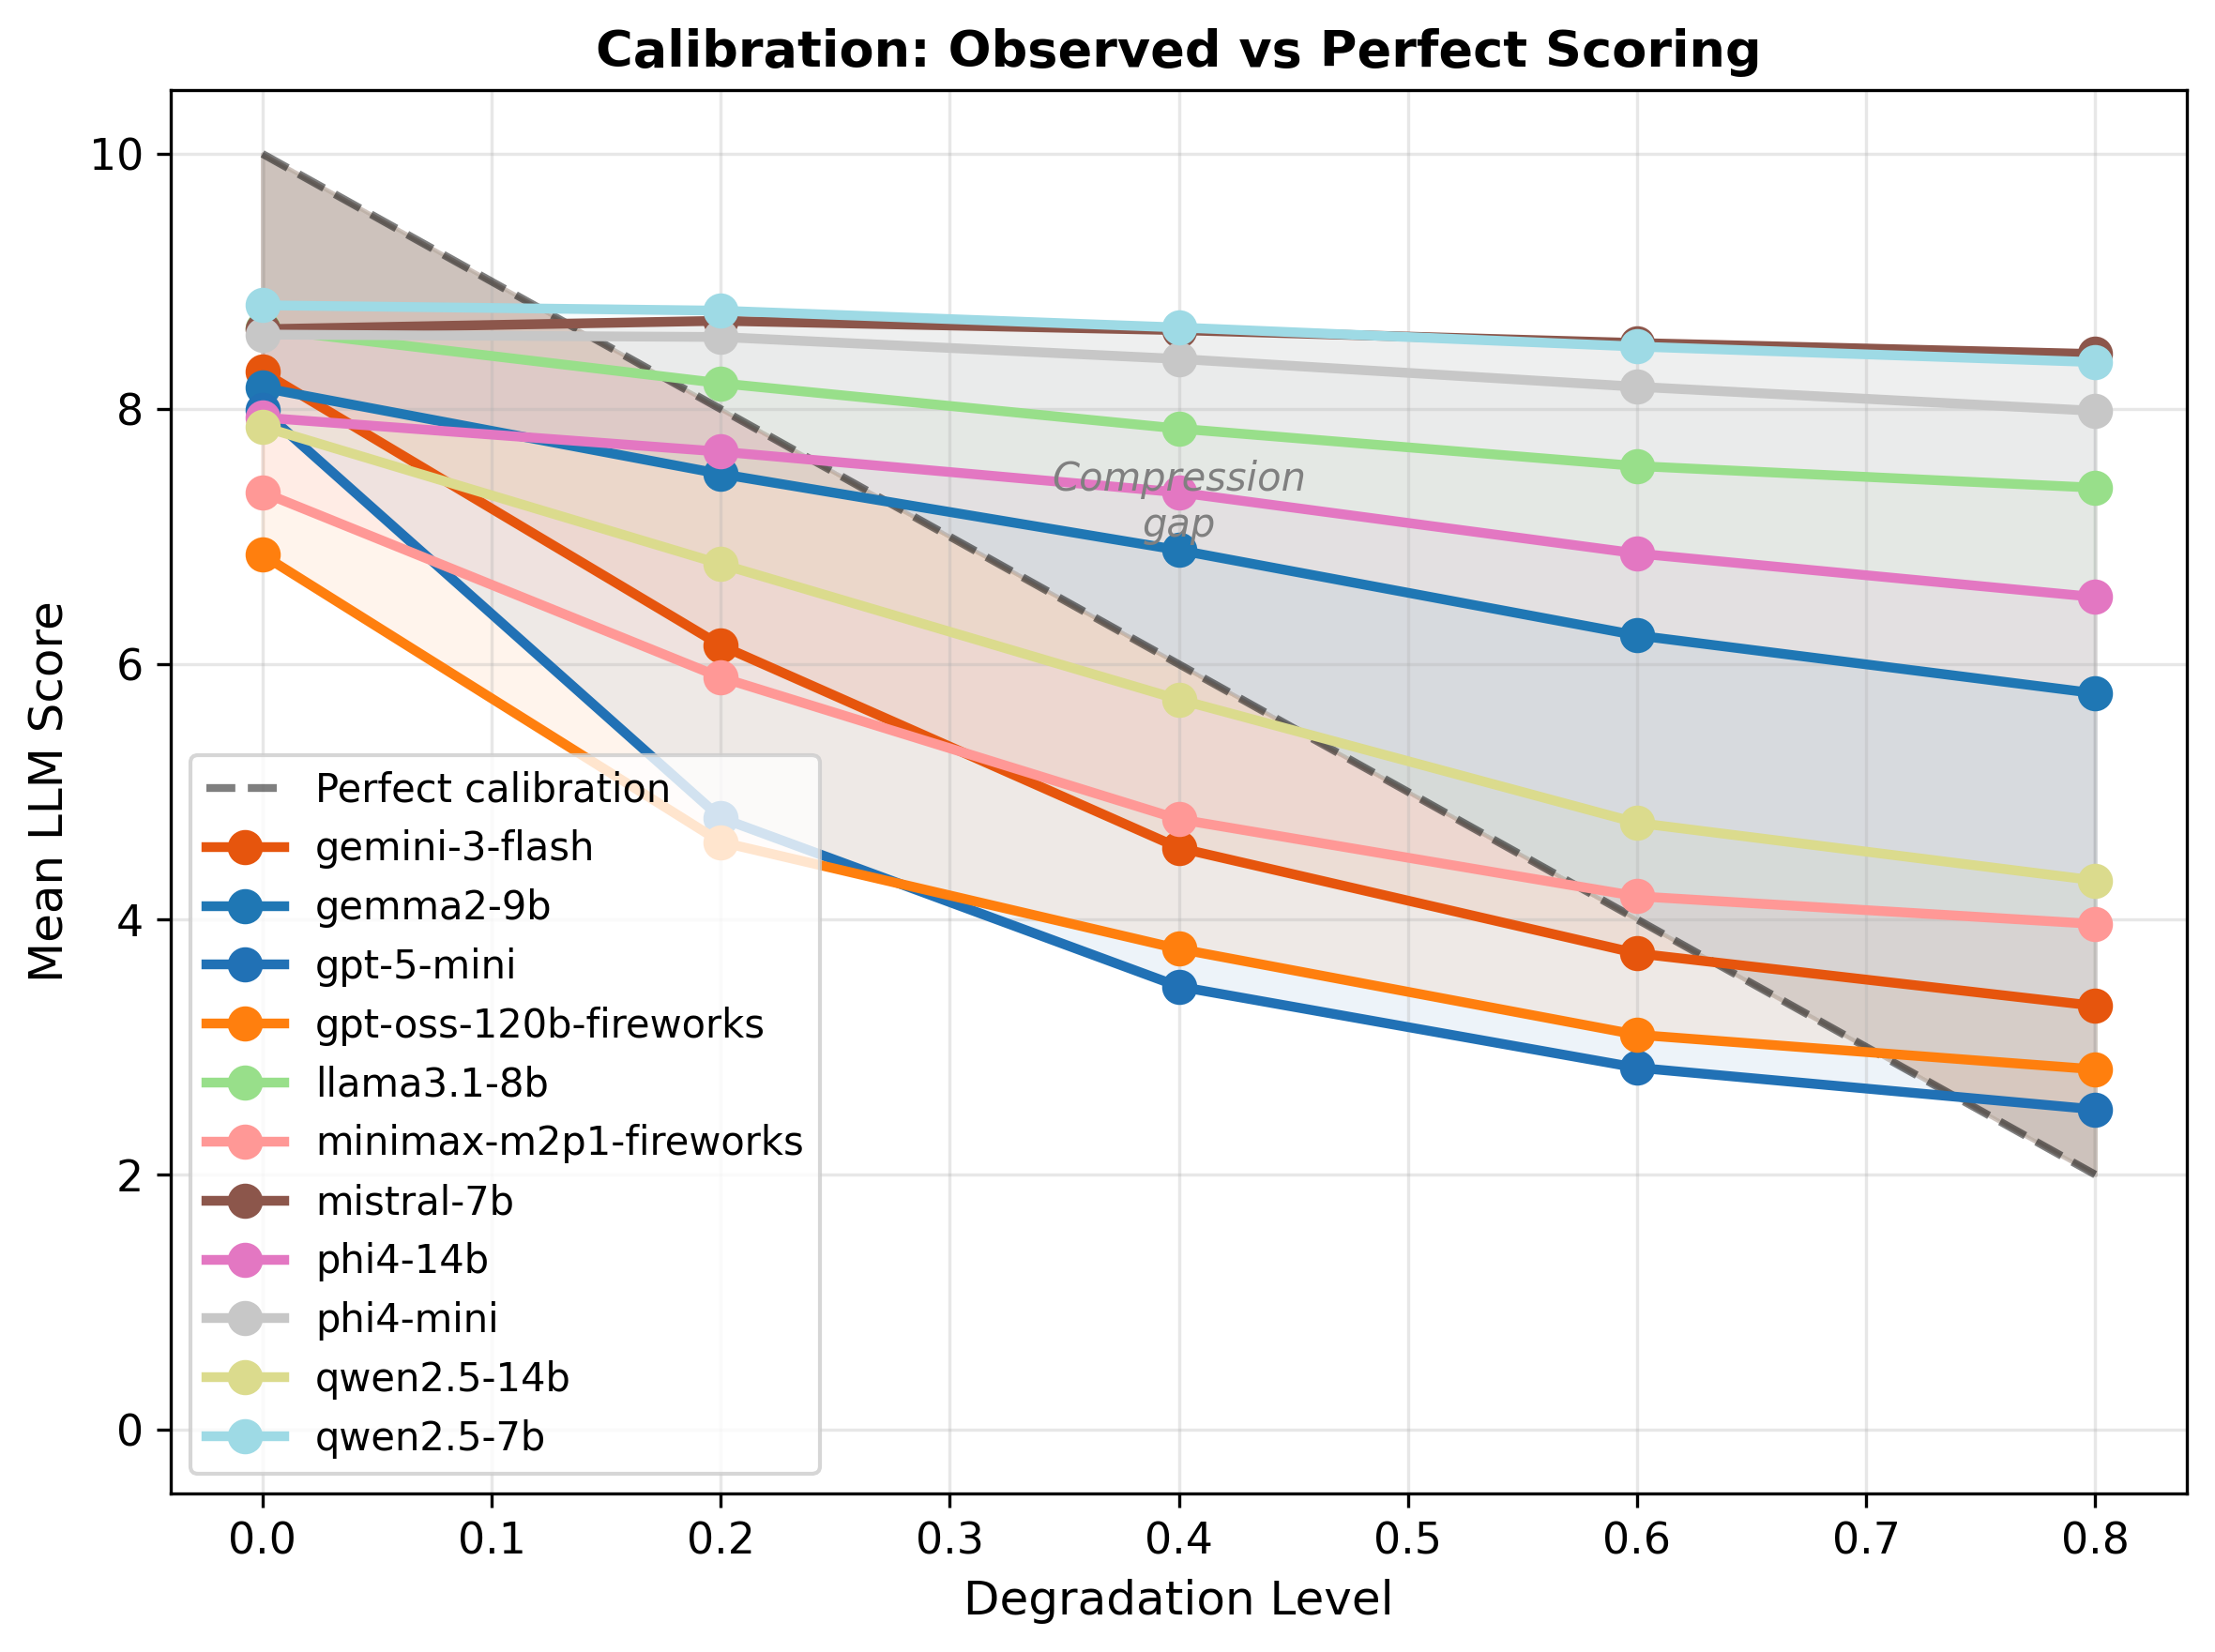
\includegraphics[width=\textwidth]{G9_calibration.png}
\caption{Calibration plot: observed mean scores vs.\ the naive calibration reference line ($S = 10(1 - \lambda)$). The shaded area represents the compression gap---the scoring range lost to boundary avoidance.}
\label{fig:calibration}
\end{figure}

\FloatBarrier
\subsection{Primary Outcome 2: Sensitivity (Regression Slopes)}

\FloatBarrier

Linear regression of score on degradation level per axis quantifies each model's sensitivity to quality changes (Table~\ref{tab:slopes}). Across all eleven models, 43 of 44 slopes are significantly negative ($p < 0.001$); the sole exception is Mistral~7B on lexical degradation ($\beta_1 = -0.03$, $p = 0.49$). The two primary models show the steepest slopes overall: information deletion produces the steepest slopes for both GPT-5~mini ($\beta_1 = -7.87$) and Gemini~3~Flash ($-7.05$), while coherence disruption produces the shallowest. Across models, sensitivity spans more than an order of magnitude: mean slopes range from $-6.46$ (GPT-5~mini) to $-0.28$ (Mistral~7B), confirming that score compression manifests not just as reduced range but as dramatically reduced sensitivity to quality changes.

\begin{table}[H]
\centering
\caption{Linear regression slopes ($\beta_1$) of score on degradation level per axis for all eleven models. All slopes are significantly negative at $p < 0.001$ except Mistral~7B lexical ($p = 0.49$, shown in gray).}
\label{tab:slopes}
\small
\begin{tabular}{@{}lccccc@{}}
\toprule
\textbf{Model} & \textbf{Grammar} & \textbf{Coherence} & \textbf{Information} & \textbf{Lexical} & \textbf{Mean} \\
\midrule
GPT-5 mini & $-6.82$ & $-4.78$ & $-7.87$ & $-6.38$ & $-6.46$ \\
Gemini 3 Flash & $-6.81$ & $-5.58$ & $-7.05$ & $-5.26$ & $-6.18$ \\
GPT-OSS 120B & $-5.16$ & $-3.36$ & $-6.08$ & $-4.55$ & $-4.79$ \\
Qwen 2.5 14B & $-5.97$ & $-1.21$ & $-6.64$ & $-4.46$ & $-4.57$ \\
MiniMax M2P1 & $-5.59$ & $-2.04$ & $-5.56$ & $-3.73$ & $-4.23$ \\
Gemma 2 9B & $-4.77$ & $-2.02$ & $-3.63$ & $-1.69$ & $-3.03$ \\
Phi-4 14B & $-2.77$ & $-0.47$ & $-3.09$ & $-0.90$ & $-1.81$ \\
Llama 3.1 8B & $-3.70$ & $-0.69$ & $-1.25$ & $-0.65$ & $-1.57$ \\
Phi-4 mini & $-1.12$ & $-0.47$ & $-1.35$ & $-0.23$ & $-0.79$ \\
Qwen 2.5 7B & $-0.75$ & $-0.54$ & $-0.84$ & $-0.22$ & $-0.59$ \\
Mistral 7B & $-0.41$ & $-0.28$ & $-0.41$ & \color{gray}{$-0.03$} & $-0.28$ \\
\bottomrule
\end{tabular}
\end{table}

The average slope across axes ranges from $-6.46$ (GPT-5~mini) to $-0.28$ (Mistral~7B). Under the naive linear reference, a slope of $-10$ would be expected (each 0.1 increase in degradation level should decrease the score by 1 point). Only the two primary models approach two-thirds of the ideal sensitivity; seven of eleven models achieve less than half. Figure~\ref{fig:forest} presents a forest plot of all slopes with 95\% confidence intervals.

\begin{figure}[!htbp]
\centering
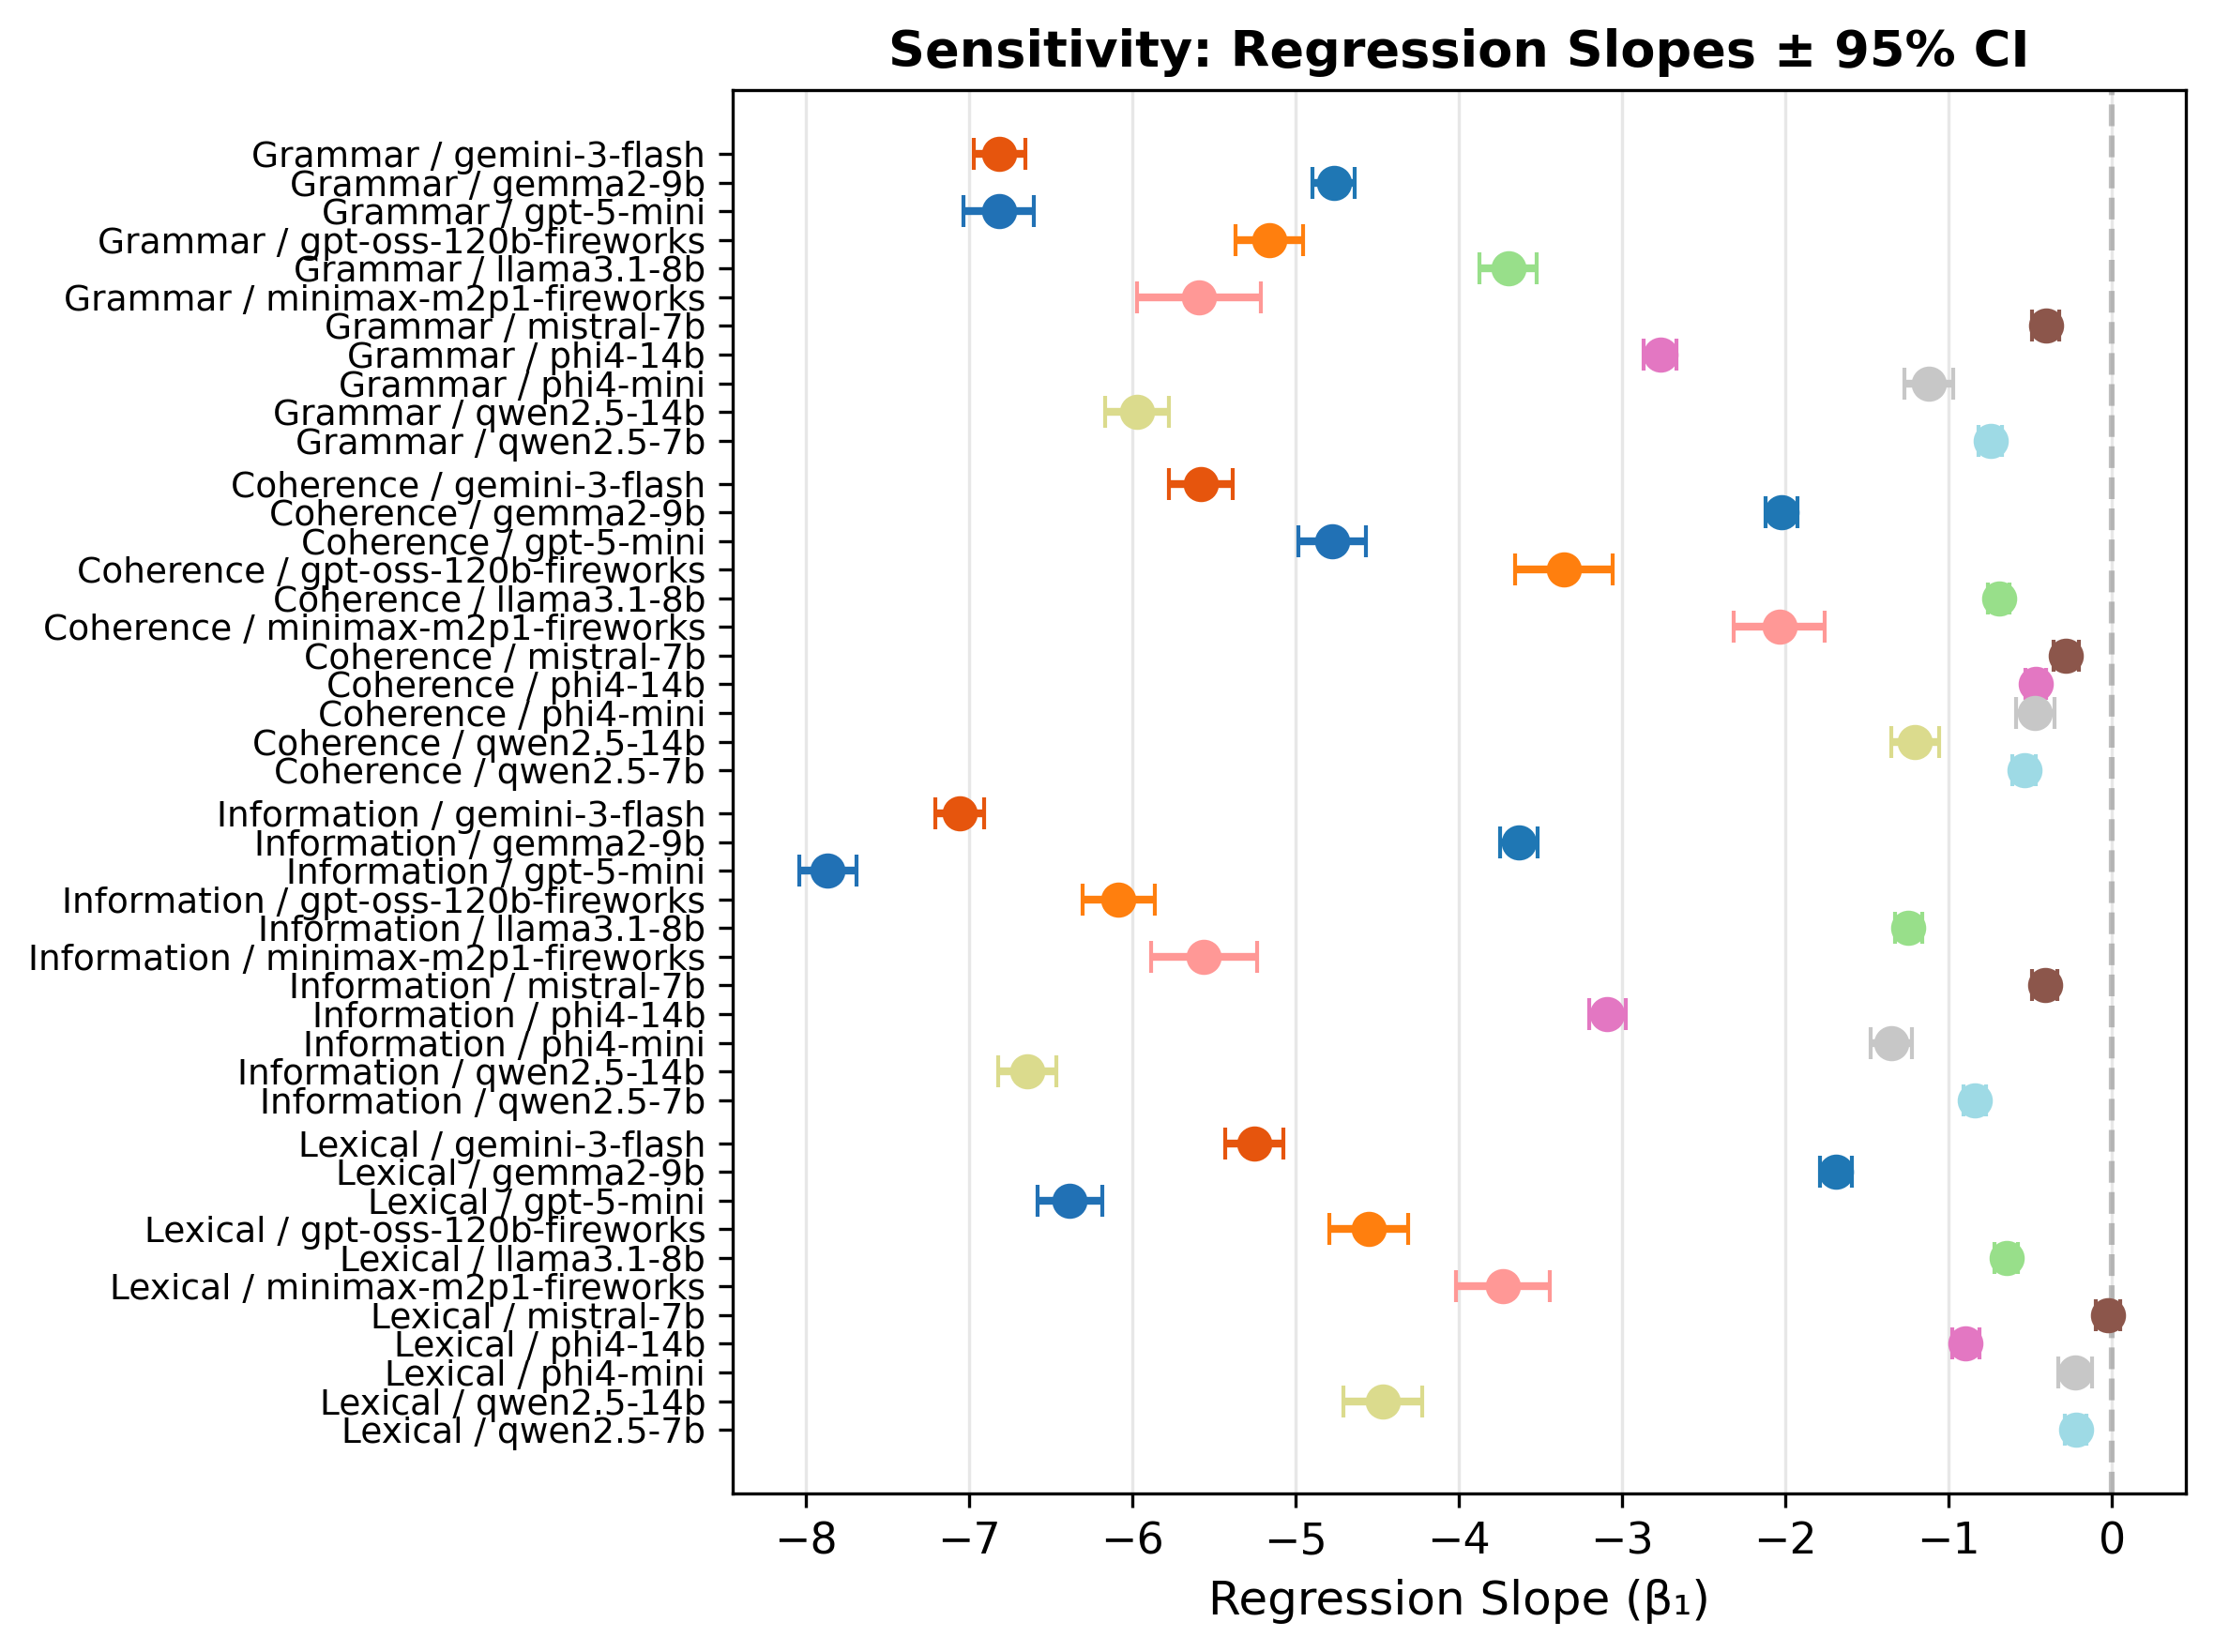
\includegraphics[width=\textwidth,height=0.65\textheight,keepaspectratio]{G8_forest_plot.png}
\caption{Forest plot of regression slopes ($\beta_1$) with 95\% CIs for each axis$\times$model combination across all eleven models. All slopes are significantly negative except Mistral~7B lexical. Information deletion elicits the steepest response across models; coherence disruption the shallowest.}
\label{fig:forest}
\end{figure}

\begin{figure}[H]
\centering
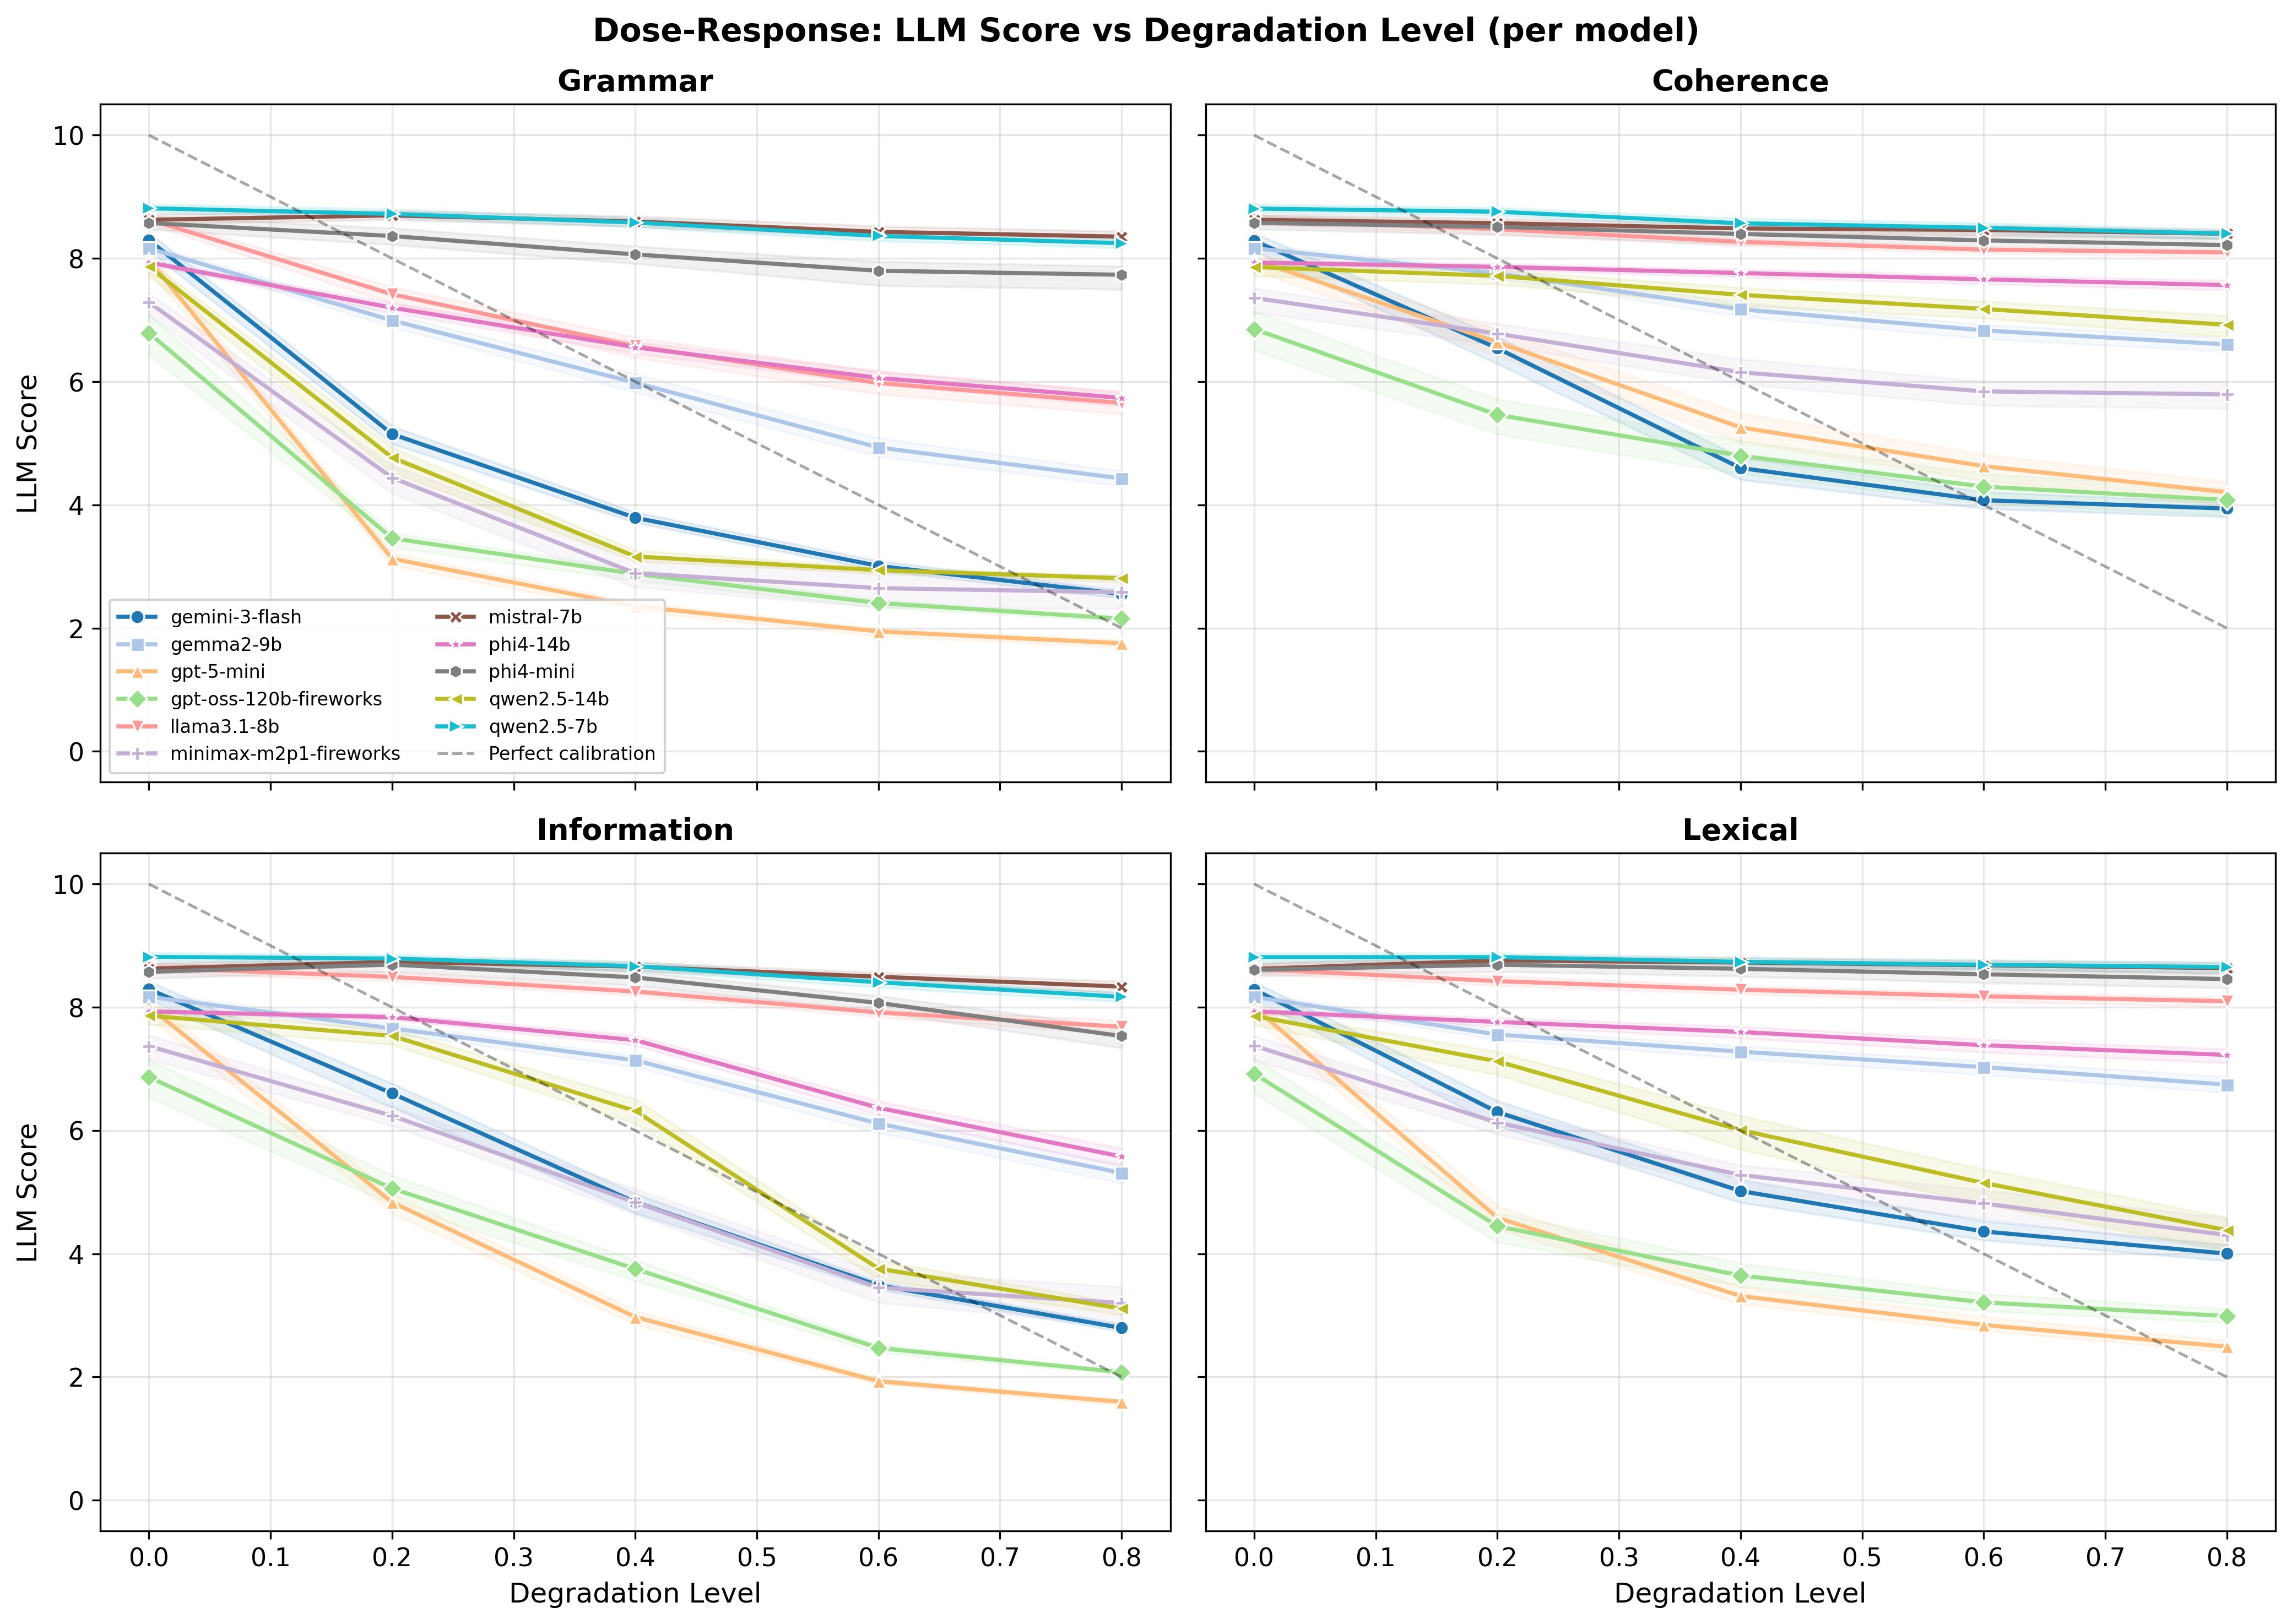
\includegraphics[width=\textwidth]{G1_dose_response.png}
\caption{Dose-response curves: mean LLM score vs.\ degradation level for each axis, with both models overlaid. Shaded bands represent 95\% block-bootstrap confidence intervals (resampling articles, 5{,}000 iterations). The dashed gray line shows the naive linear reference. Note the concave shape---sensitivity diminishes at higher degradation levels.}
\label{fig:doseresponse}
\end{figure}

\begin{figure}[H]
\centering
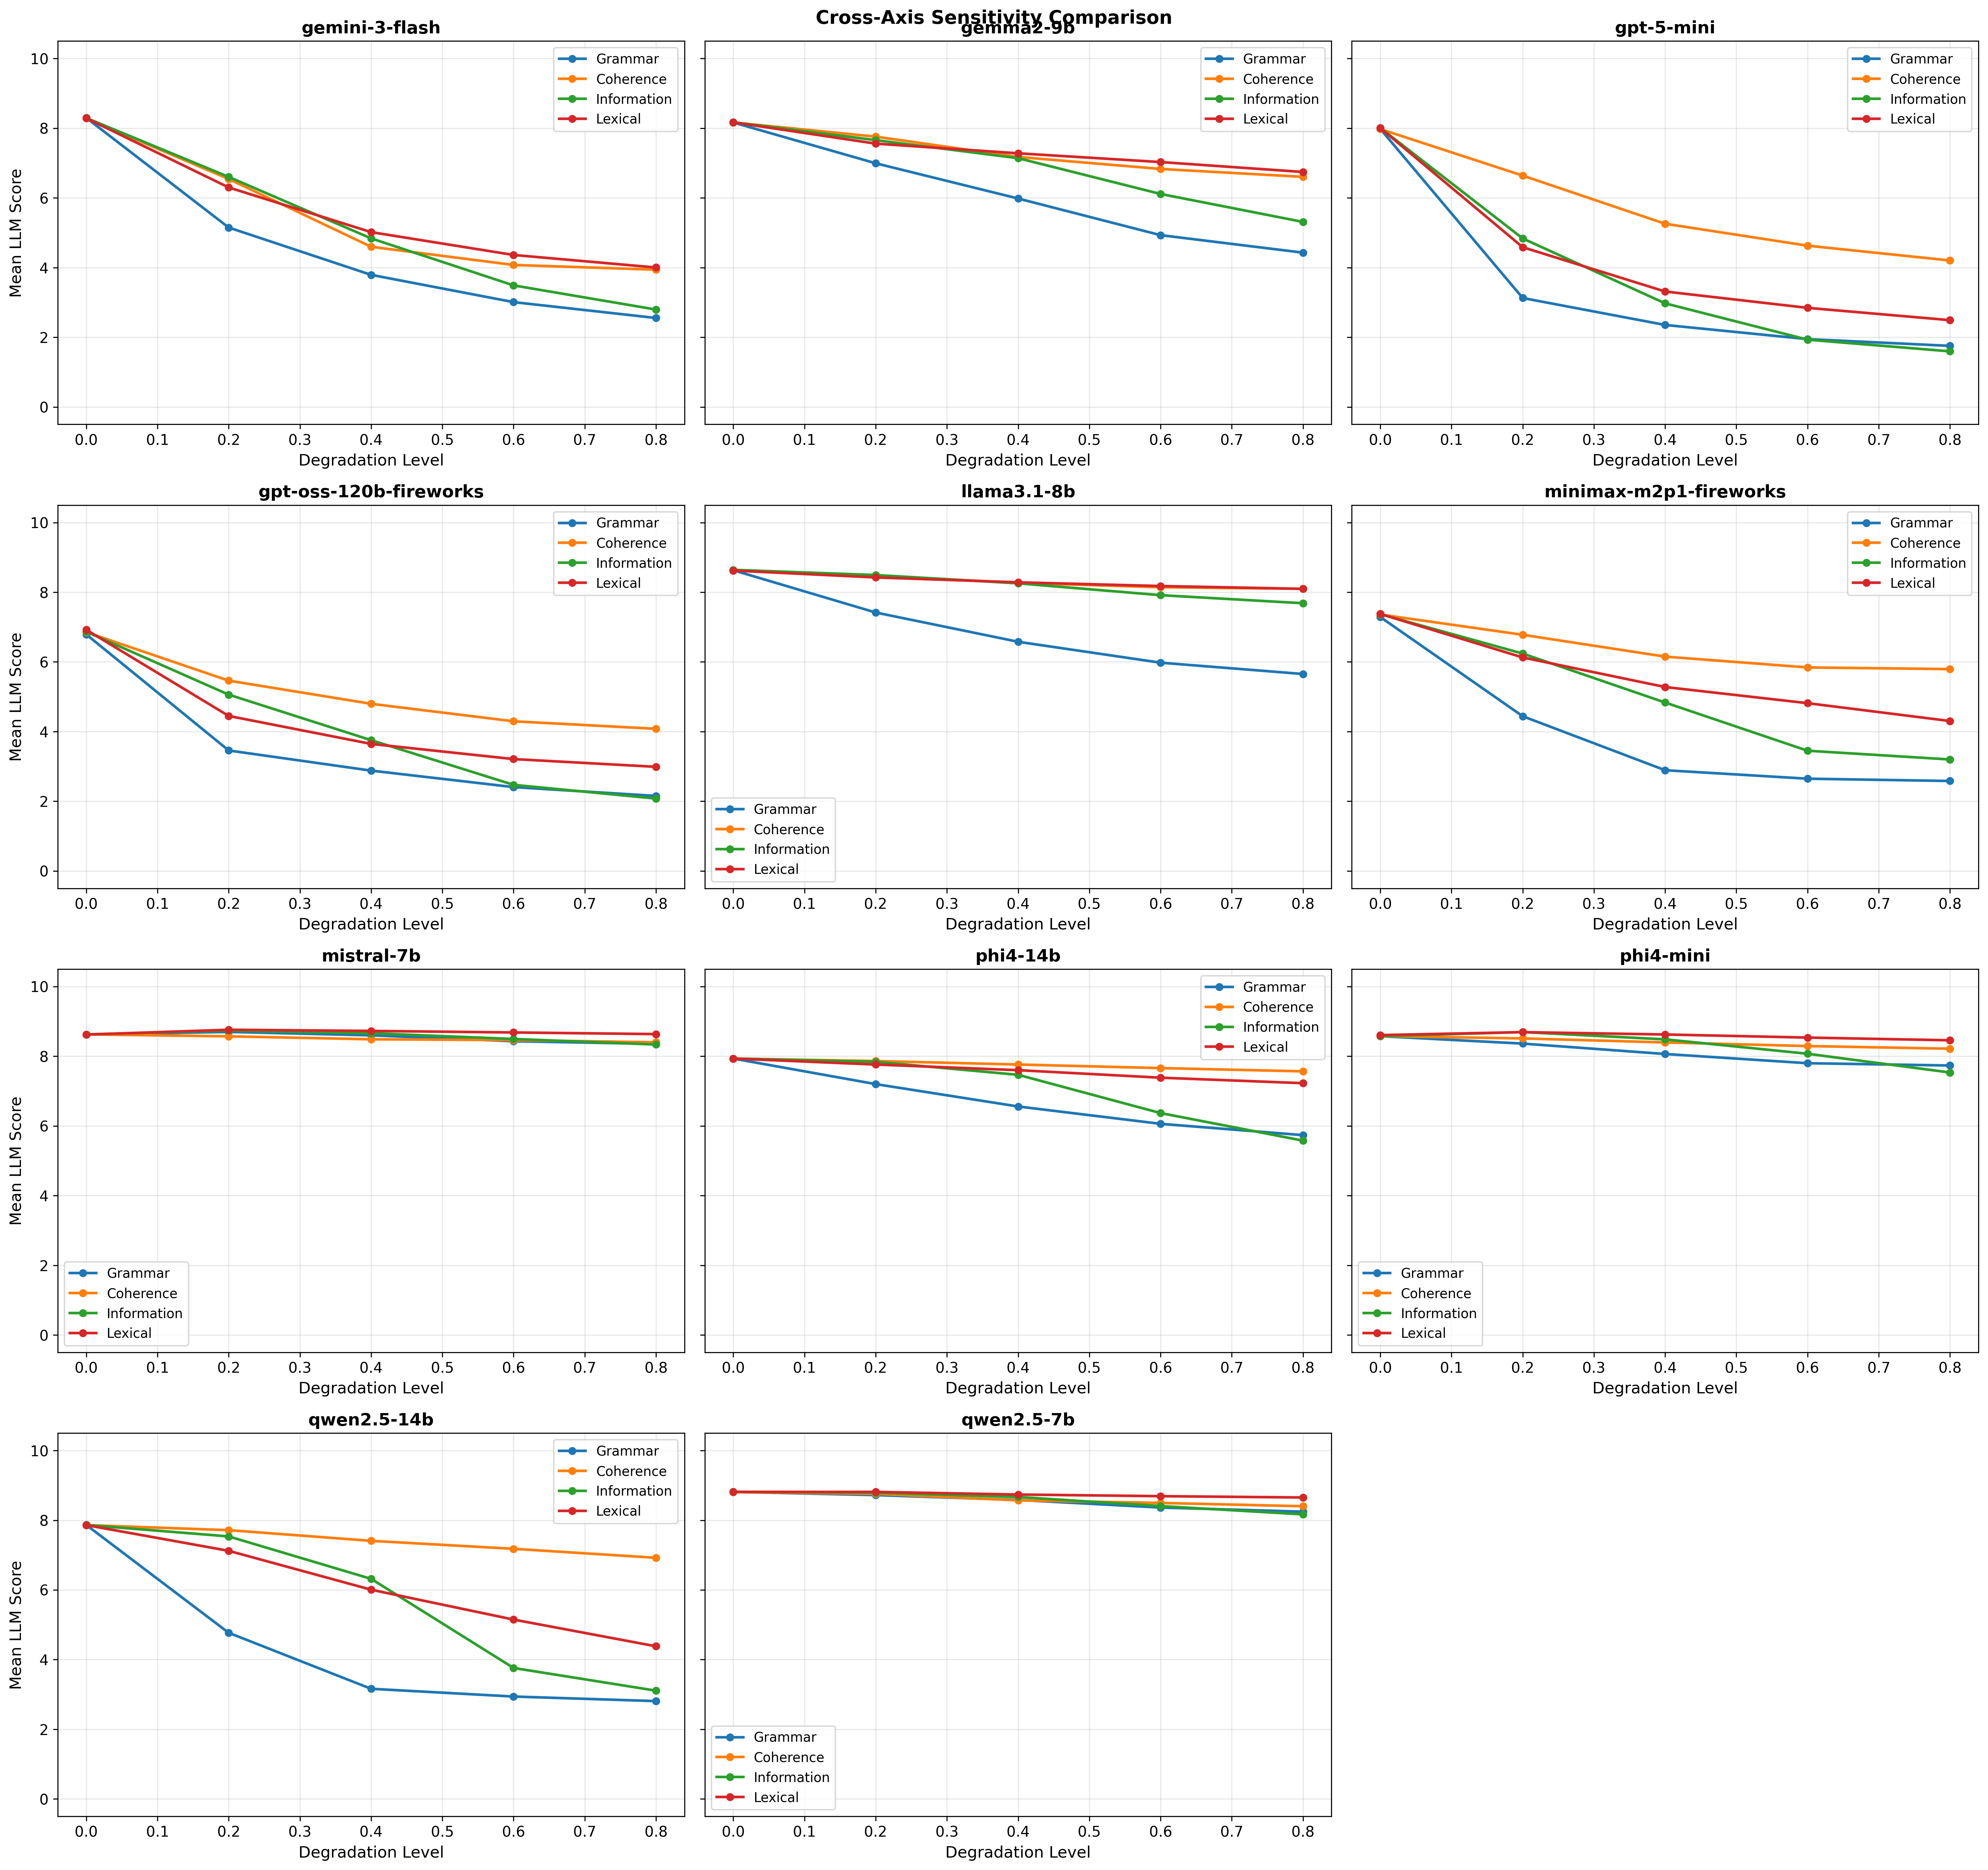
\includegraphics[width=\textwidth]{G2_cross_axis.png}
\caption{Cross-axis sensitivity comparison per model. Both models are most sensitive to information deletion and least sensitive to coherence disruption, though the magnitude of the gap differs.}
\label{fig:crossaxis}
\end{figure}

\subsection{Non-linearity}

The dose-response curves (Figure~\ref{fig:doseresponse}) reveal visibly concave trajectories for the primary models. A nested $F$-test comparing linear and quadratic regression models confirms significant quadratic terms for most axis$\times$model combinations (Table~\ref{tab:nonlin}). Among the two primary models, all eight combinations are highly significant ($p < 10^{-20}$). Across all eleven models, 32 of 44 combinations show significant quadratic effects ($F > 3.84$, $p < 0.05$). All significant quadratic coefficients are positive, indicating concave dose-response curves: sensitivity is highest at low degradation levels and diminishes as quality approaches the floor. Models with very low CRs (Mistral~7B, Qwen~2.5~7B, Phi-4~mini) show weak or absent quadratic effects on several axes, reflecting their overall insensitivity to degradation.

\begin{table}[H]
\centering
\caption{Non-linearity: $F$-statistic for quadratic term across all eleven models. Bold values indicate $p < 0.001$; ``---'' indicates $F < 1$ (not significant).}
\label{tab:nonlin}
\small
\begin{tabular}{@{}lcccc@{}}
\toprule
\textbf{Model} & \textbf{Grammar} & \textbf{Coherence} & \textbf{Info} & \textbf{Lexical} \\
\midrule
GPT-5 mini & \textbf{3{,}556} & \textbf{110} & \textbf{1{,}640} & \textbf{1{,}335} \\
Gemini 3 Flash & \textbf{1{,}757} & \textbf{463} & \textbf{192} & \textbf{382} \\
GPT-OSS 120B & \textbf{880} & \textbf{49} & \textbf{120} & \textbf{317} \\
Qwen 2.5 14B & \textbf{1{,}683} & --- & \textbf{86} & --- \\
MiniMax M2P1 & \textbf{254} & \textbf{17} & \textbf{21} & \textbf{29} \\
Gemma 2 9B & \textbf{73} & \textbf{25} & \textbf{63} & \textbf{33} \\
Phi-4 14B & \textbf{63} & --- & \textbf{279} & --- \\
Llama 3.1 8B & \textbf{96} & \textbf{13} & 7 & 10 \\
Phi-4 mini & 3 & --- & \textbf{105} & 8 \\
Qwen 2.5 7B & 2 & --- & \textbf{44} & --- \\
Mistral 7B & \textbf{14} & --- & \textbf{45} & \textbf{19} \\
\bottomrule
\end{tabular}
\end{table}

\subsection{Monotonicity}

Kendall's $\tau$ confirms monotonic relationships between degradation level and score across all models and axes (Table~\ref{tab:tau}). For the primary models, values range from $\tau = -0.57$ (GPT, coherence) to $\tau = -0.83$ (GPT, information). The pattern is consistent across the model landscape: information and grammar axes generally elicit the strongest monotonic responses, while coherence and lexical axes are weaker. Severely compressed models (Mistral~7B, Phi-4~mini) show notably weaker monotonicity, with $|\tau| < 0.20$ on several axes, indicating that these models barely distinguish between degradation levels.

\begin{table}[H]
\centering
\caption{Kendall's $\tau$ between degradation level and score for all eleven models. All values are significant at $p < 10^{-4}$ except Mistral~7B lexical ($\tau = -0.005$, $p = 0.49$).}
\label{tab:tau}
\small
\begin{tabular}{@{}lcccc@{}}
\toprule
\textbf{Model} & \textbf{Grammar} & \textbf{Coherence} & \textbf{Info} & \textbf{Lexical} \\
\midrule
GPT-5 mini & $-0.733$ & $-0.568$ & $-0.827$ & $-0.675$ \\
Gemini 3 Flash & $-0.818$ & $-0.636$ & $-0.818$ & $-0.661$ \\
GPT-OSS 120B & $-0.673$ & $-0.408$ & $-0.700$ & $-0.528$ \\
Qwen 2.5 14B & $-0.708$ & $-0.382$ & $-0.761$ & $-0.559$ \\
Gemma 2 9B & $-0.768$ & $-0.585$ & $-0.747$ & $-0.524$ \\
MiniMax M2P1 & $-0.487$ & $-0.270$ & $-0.516$ & $-0.420$ \\
Phi-4 14B & $-0.700$ & $-0.264$ & $-0.716$ & $-0.375$ \\
Llama 3.1 8B & $-0.605$ & $-0.358$ & $-0.506$ & $-0.315$ \\
Phi-4 mini & $-0.265$ & $-0.136$ & $-0.348$ & $-0.058$ \\
Qwen 2.5 7B & $-0.351$ & $-0.267$ & $-0.399$ & $-0.128$ \\
Mistral 7B & $-0.172$ & $-0.129$ & $-0.181$ & $-0.005$ \\
\bottomrule
\end{tabular}
\end{table}

\FloatBarrier
\subsection{Mixed-Effects Model}
\label{sec:mixedeffects}

The following two subsections focus on the two primary frontier models (GPT-5~mini and Gemini~3~Flash) for detailed interaction analysis. These models were selected because they are the highest-performing API models from different providers, both achieving CRs above 0.60 and Spearman $\rho > 0.70$ (Table~\ref{tab:compression}), making their comparison the most informative for understanding how two well-calibrated but architecturally distinct models differ in their scoring behavior. The mixed-effects specification requires exactly two model levels to estimate the three-way interaction, and the inter-model agreement metrics are inherently pairwise.

A three-way linear mixed-effects model with the specification

\begin{equation}
    S_{ijk} \sim \lambda \times \mathrm{Axis} \times \mathrm{Model} + (1 + \lambda \mid \text{Article})
\end{equation}

\noindent converged successfully with random intercepts and slopes. Key findings (full coefficients in Supplementary Material):

\begin{itemize}[nosep]
    \item The main effect of degradation level is large and negative ($\beta = -4.76$, $z = -45.6$, $p < 10^{-300}$).
    \item The main effect of model (Gemini vs.\ GPT) is non-significant at the intercept ($\beta = +0.07$, $p = 0.25$), indicating comparable baseline scoring.
    \item All axis effects are significant, with grammar showing the largest intercept reduction ($\beta = -1.49$, $z = -25.1$).
    \item Critically, the three-way $\mathrm{Level} \times \mathrm{Axis} \times \mathrm{Model}$ interactions are all significant, confirming that the two models differ in their axis-specific sensitivity profiles. The largest three-way interaction is $\mathrm{Level} \times \mathrm{Lexical} \times \mathrm{Gemini}$ ($\beta = +1.93$, $z = +11.2$), indicating that Gemini is substantially less sensitive to lexical degradation than GPT.
    \item Random effects: article-level intercept variance $= 0.54$; article-level slope variance $= 0.49$, indicating meaningful between-article variability in both baseline score and degradation sensitivity.
\end{itemize}

\FloatBarrier
\subsection{Primary Outcome 3: Inter-Model Comparison}

\begin{table}[t]
\centering
\caption{Inter-model agreement and systematic bias.}
\label{tab:intermodel}
\begin{tabular}{@{}lr@{}}
\toprule
\textbf{Metric} & \textbf{Value} \\
\midrule
Pearson $r$ & 0.836 \\
Spearman $\rho$ & 0.817 \\
Median paired difference (Gem $-$ GPT) & +1.0 \\
Mean paired difference & +0.89 \\
Wilcoxon $W$ & 3{,}541{,}954 \\
Rank-biserial $r$ & +0.705 \\
Cohen's weighted $\kappa$ (quadratic) & 0.772 \\
\bottomrule
\end{tabular}
\end{table}

Despite high overall agreement (Table~\ref{tab:intermodel}), Gemini~3~Flash scores systematically higher than GPT-5~mini by a median of +1 point ($p < 10^{-300}$). This bias is present across all four degradation axes, with the largest median difference on grammar, information, and lexical ($+1$) and the smallest on coherence ($0$). Per-axis Wilcoxon tests are all significant after Benjamini-Hochberg correction. Figure~\ref{fig:scatter} shows the inter-model agreement scatter, and Figure~\ref{fig:paireddiff} shows the distribution of paired differences.

\begin{figure}[!htbp]
\centering
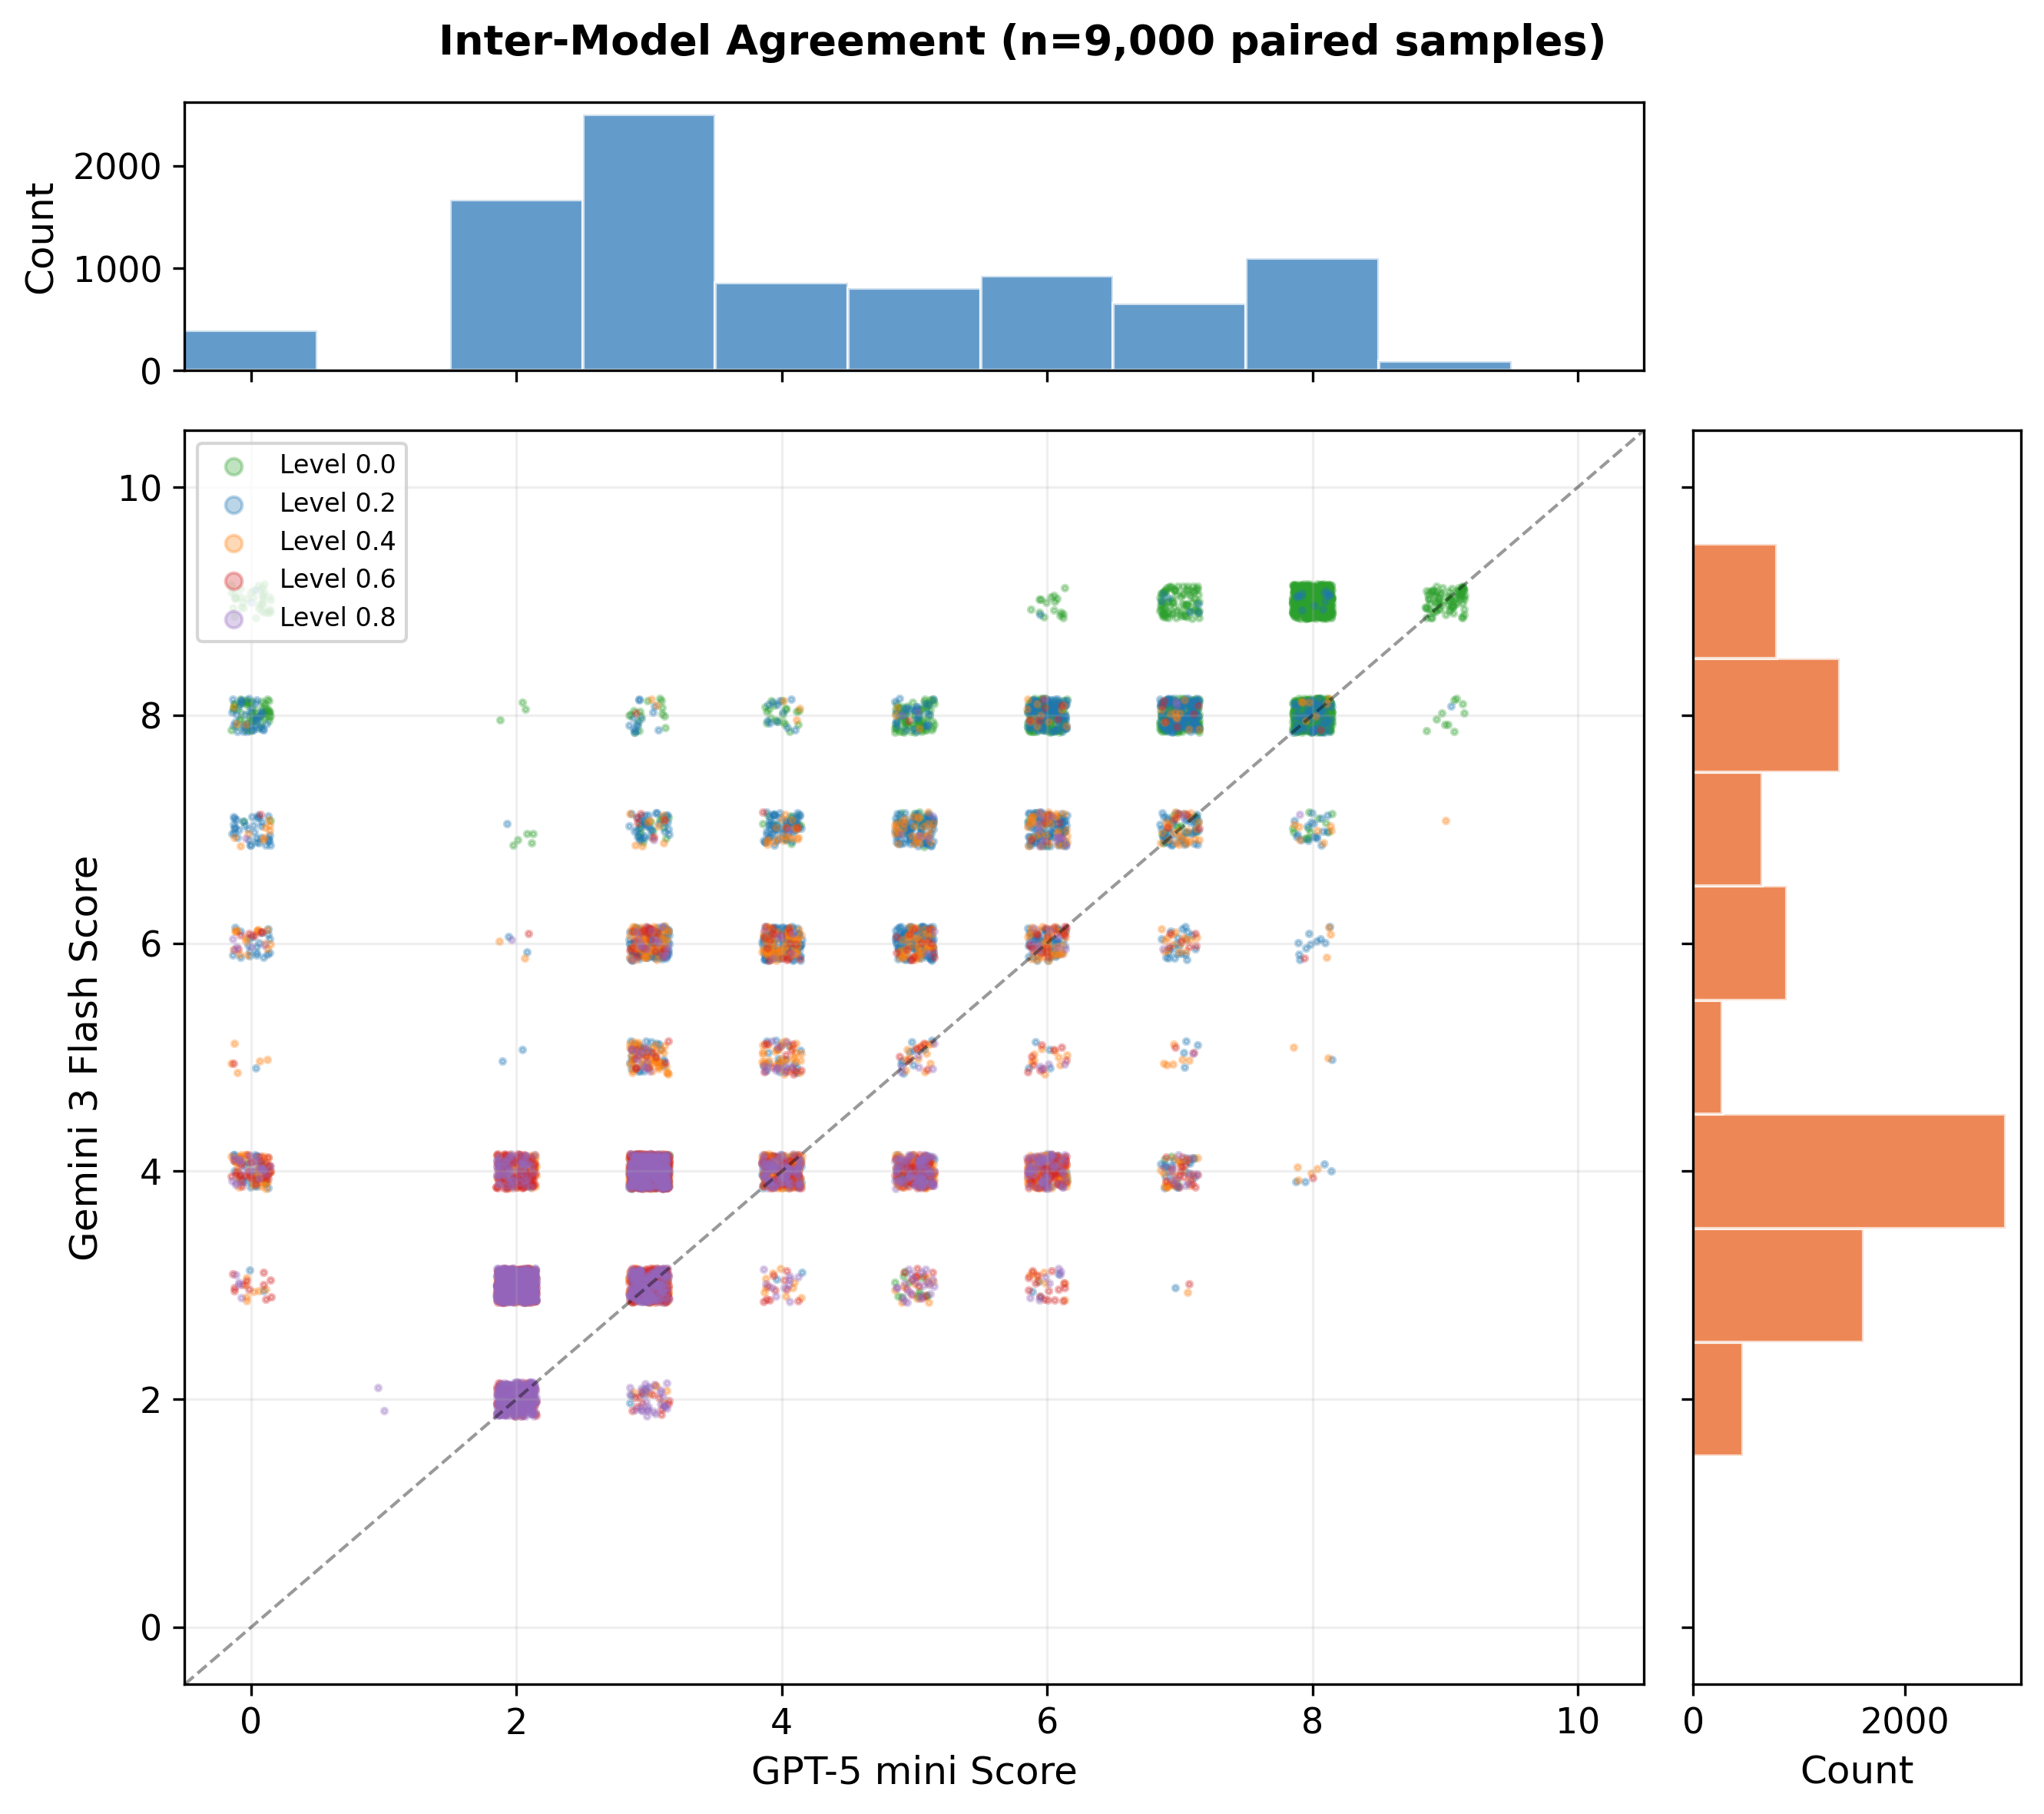
\includegraphics[width=\textwidth]{G10_inter_model_scatter.png}
\caption{Inter-model agreement scatter plot ($n = 9{,}000$ paired samples). Each point is one sample, jittered, colored by degradation level. The dashed line is the identity line; points above it indicate Gemini scored higher. Marginal histograms show each model's score distribution.}
\label{fig:scatter}
\end{figure}

\begin{figure}[H]
\centering
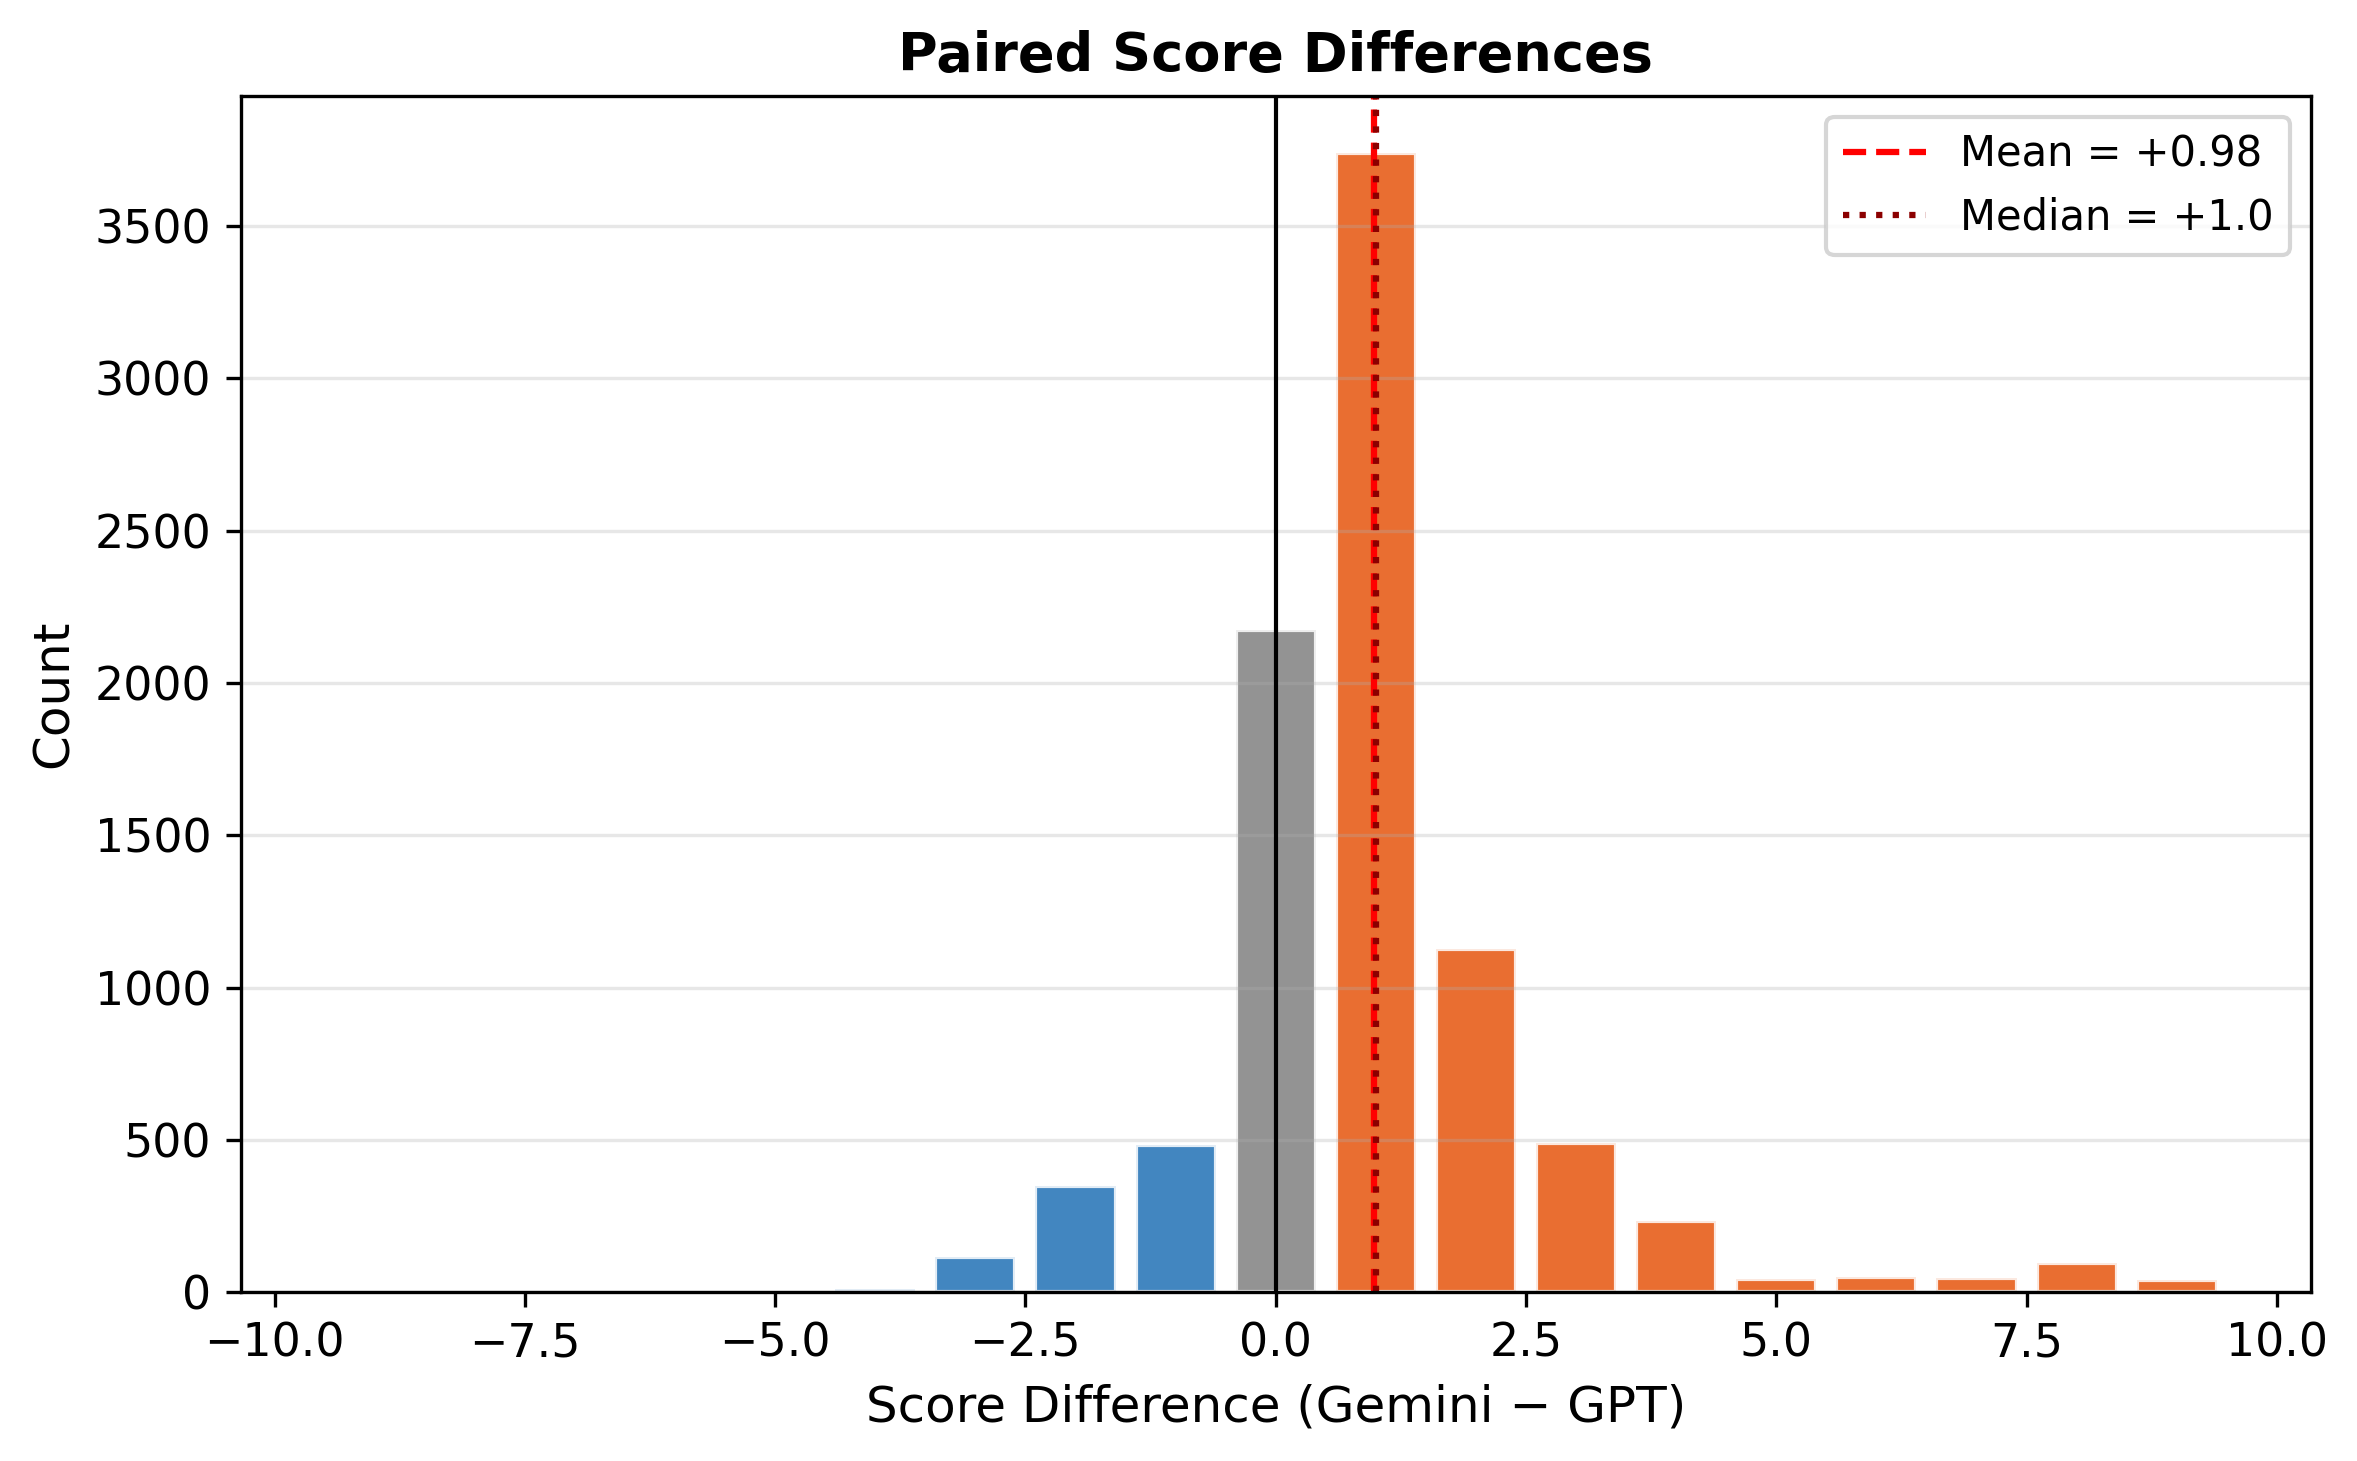
\includegraphics[width=\textwidth]{G11_paired_diff.png}
\caption{Distribution of paired score differences (Gemini $-$ GPT). The distribution is right-shifted with a median of $+1$ and mean of $+0.89$, confirming systematic positive bias.}
\label{fig:paireddiff}
\end{figure}

\subsection{Variance Heterogeneity}

Levene's test confirms significant variance heterogeneity across degradation levels for all eleven models. Among the primary models, GPT-5~mini ($W = 136.6$, $p < 10^{-113}$) and Gemini~3~Flash ($W = 183.6$, $p < 10^{-151}$) both show the pattern. Across all models, Levene's $W$ ranges from 44.7 (Llama~3.1~8B) to 589.2 (Phi-4~14B), all highly significant. Score variance peaks at $\lambda = 0.2$ for most models and is lowest at $\lambda = 0.0$, consistent with a ``fan-out-then-in'' pattern reflecting ceiling compression at low degradation and floor compression at high degradation. The per-level score distributions (Figure~\ref{fig:perlevel}), boxplots (Figure~\ref{fig:boxplots}), and violin plots (Figure~\ref{fig:violins}) all visualize this heteroscedasticity.

\begin{figure}[!htbp]
\centering
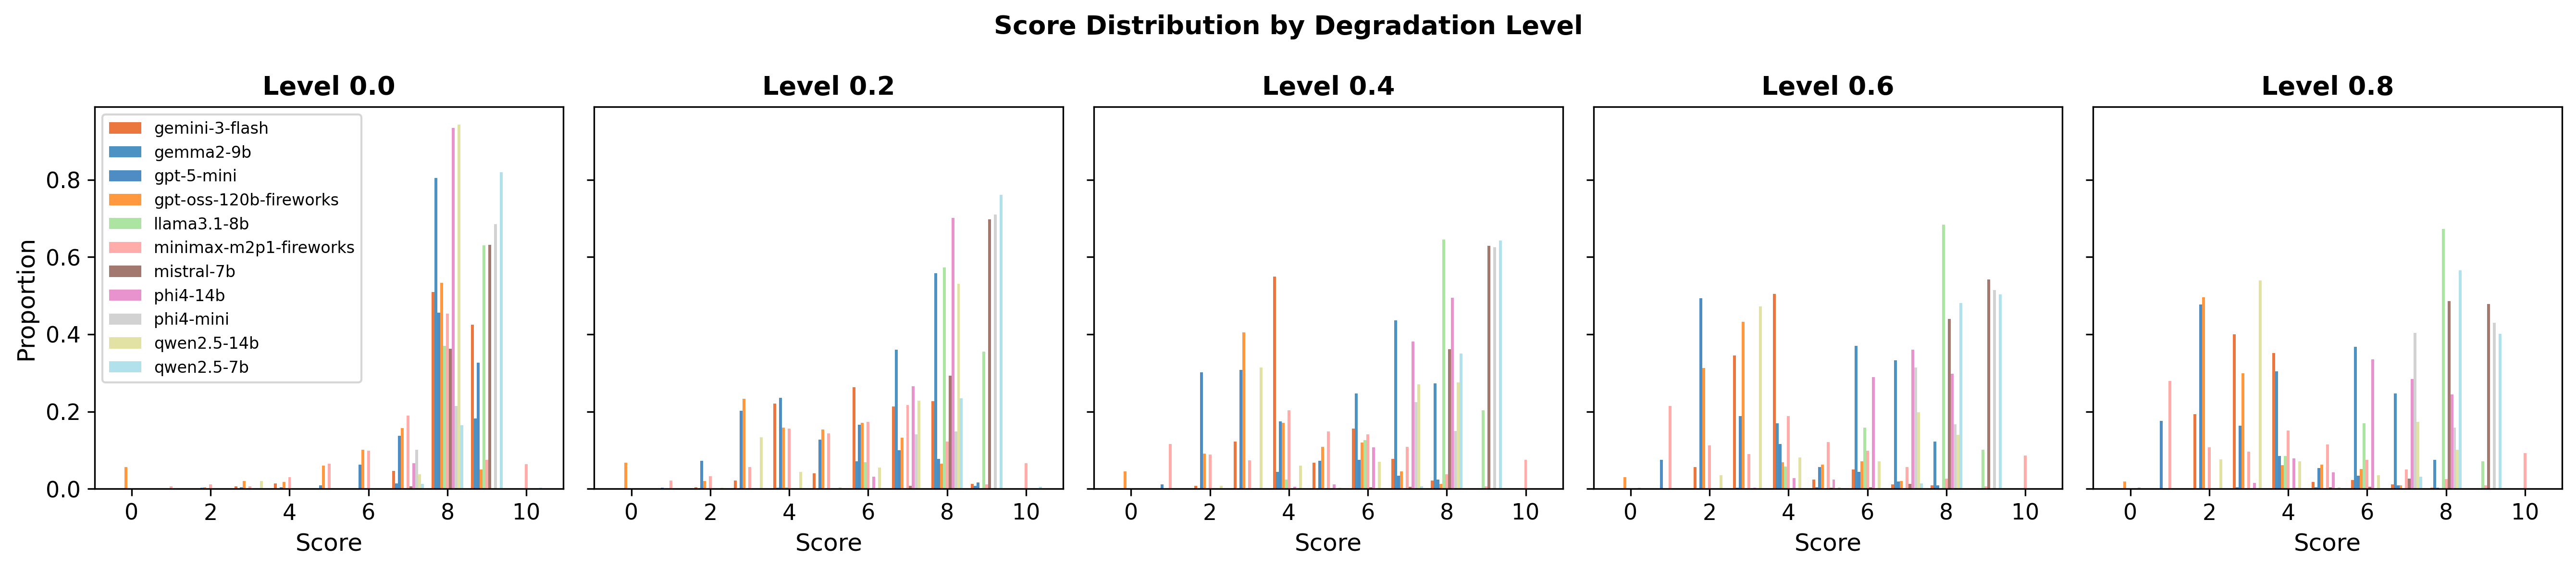
\includegraphics[width=\textwidth]{G5_per_level_dist.png}
\caption{Score distributions by degradation level. At $\lambda = 0.0$, scores concentrate tightly at 8--9. As degradation increases, the distribution shifts leftward and broadens, then reconcentrates at 2--4 by $\lambda = 0.8$.}
\label{fig:perlevel}
\end{figure}

Additional visualizations of these distributions---including boxplots by axis and level (Figure~\ref{fig:boxplots}) and violin plots by level and model (Figure~\ref{fig:violins})---are provided in the Supplementary Material.

\FloatBarrier
\subsection{Calibration Recovery}
\label{sec:calibration}

The compression results above raise a natural question: can the bias be corrected post hoc? We investigate using the two primary models, as the calibration experiment requires held-out test data with proxy ground truth and was designed as part of the initial two-model study. The findings generalize to the broader model set through the mitigation experiments in Section~\ref{sec:mitresults}. We investigate whether a learned calibration function can recover the lost scoring range. We split the 150 source articles into a training set (112 articles, 7{,}140 samples) and a held-out test set (28 articles, 1{,}860 samples), stratified by category, and fit three calibration functions on the training set: an affine transform $\hat{S} = aS_{\text{raw}} + b$, a four-parameter sigmoid $\hat{S} = d + c / (1 + e^{-a(S_{\text{raw}} - b)})$, and isotonic regression (a nonparametric monotonic mapping that serves as an upper bound on what any monotonic calibration can achieve). We evaluate on the held-out test set to avoid overfitting.

Table~\ref{tab:calibration} reports the results. Affine calibration reduces the root-mean-square error (RMSE) against the ideal score by 27\% for GPT-5~mini ($2.56 \to 1.87$) and 12\% for Gemini~3~Flash ($1.82 \to 1.60$). Strikingly, neither the sigmoid nor the isotonic regression---the best possible monotonic calibration---offers meaningful improvement over the simple two-parameter affine. This convergence demonstrates two things: (i)~the compression is well approximated as a linear distortion, and (ii)~the residual RMSE of $\sim$1.6--1.9 points represents an irreducible floor arising from the models' imperfect rank discrimination, which no monotonic transform can correct. Rank-order correlations (Kendall $\tau$, Spearman $\rho$) are unchanged by all calibrations, as expected for monotonic transforms.

\begin{table}[t]
\centering
\caption{Calibration recovery on held-out test set (28 articles, 1{,}860 samples). RMSE is computed against the ideal score $S^* = 10(1 - \lambda)$. Isotonic regression provides a nonparametric upper bound.}
\label{tab:calibration}
\begin{tabular}{@{}llcccc@{}}
\toprule
\textbf{Model} & \textbf{Calib.} & \textbf{RMSE} & $\Delta$\textbf{RMSE} & \textbf{Kendall} $\tau$ & \textbf{Spearman} $\rho$ \\
\midrule
\multirow{3}{*}{GPT-5 mini}
  & Raw      & 2.56 & ---    & 0.623 & 0.734 \\
  & Affine   & 1.87 & $-$27\% & 0.623 & 0.734 \\
  & Isotonic & 1.87 & $-$27\% & 0.627 & 0.733 \\
\midrule
\multirow{3}{*}{Gemini 3 Flash}
  & Raw      & 1.82 & ---    & 0.728 & 0.821 \\
  & Affine   & 1.60 & $-$12\% & 0.728 & 0.821 \\
  & Isotonic & 1.59 & $-$13\% & 0.728 & 0.821 \\
\bottomrule
\end{tabular}
\end{table}

Figure~\ref{fig:calibrecovery} visualizes the effect: the calibrated dose-response curves are pulled closer to the ideal line $S = 10(1 - \lambda)$, narrowing the shaded compression gap, though a residual error of 1.6--1.9 RMSE points remains even after calibration. This residual reflects the models' imperfect rank discrimination---their inability to linearly separate degradation levels---which no monotonic transform can correct.

\begin{figure}[!htbp]
\centering
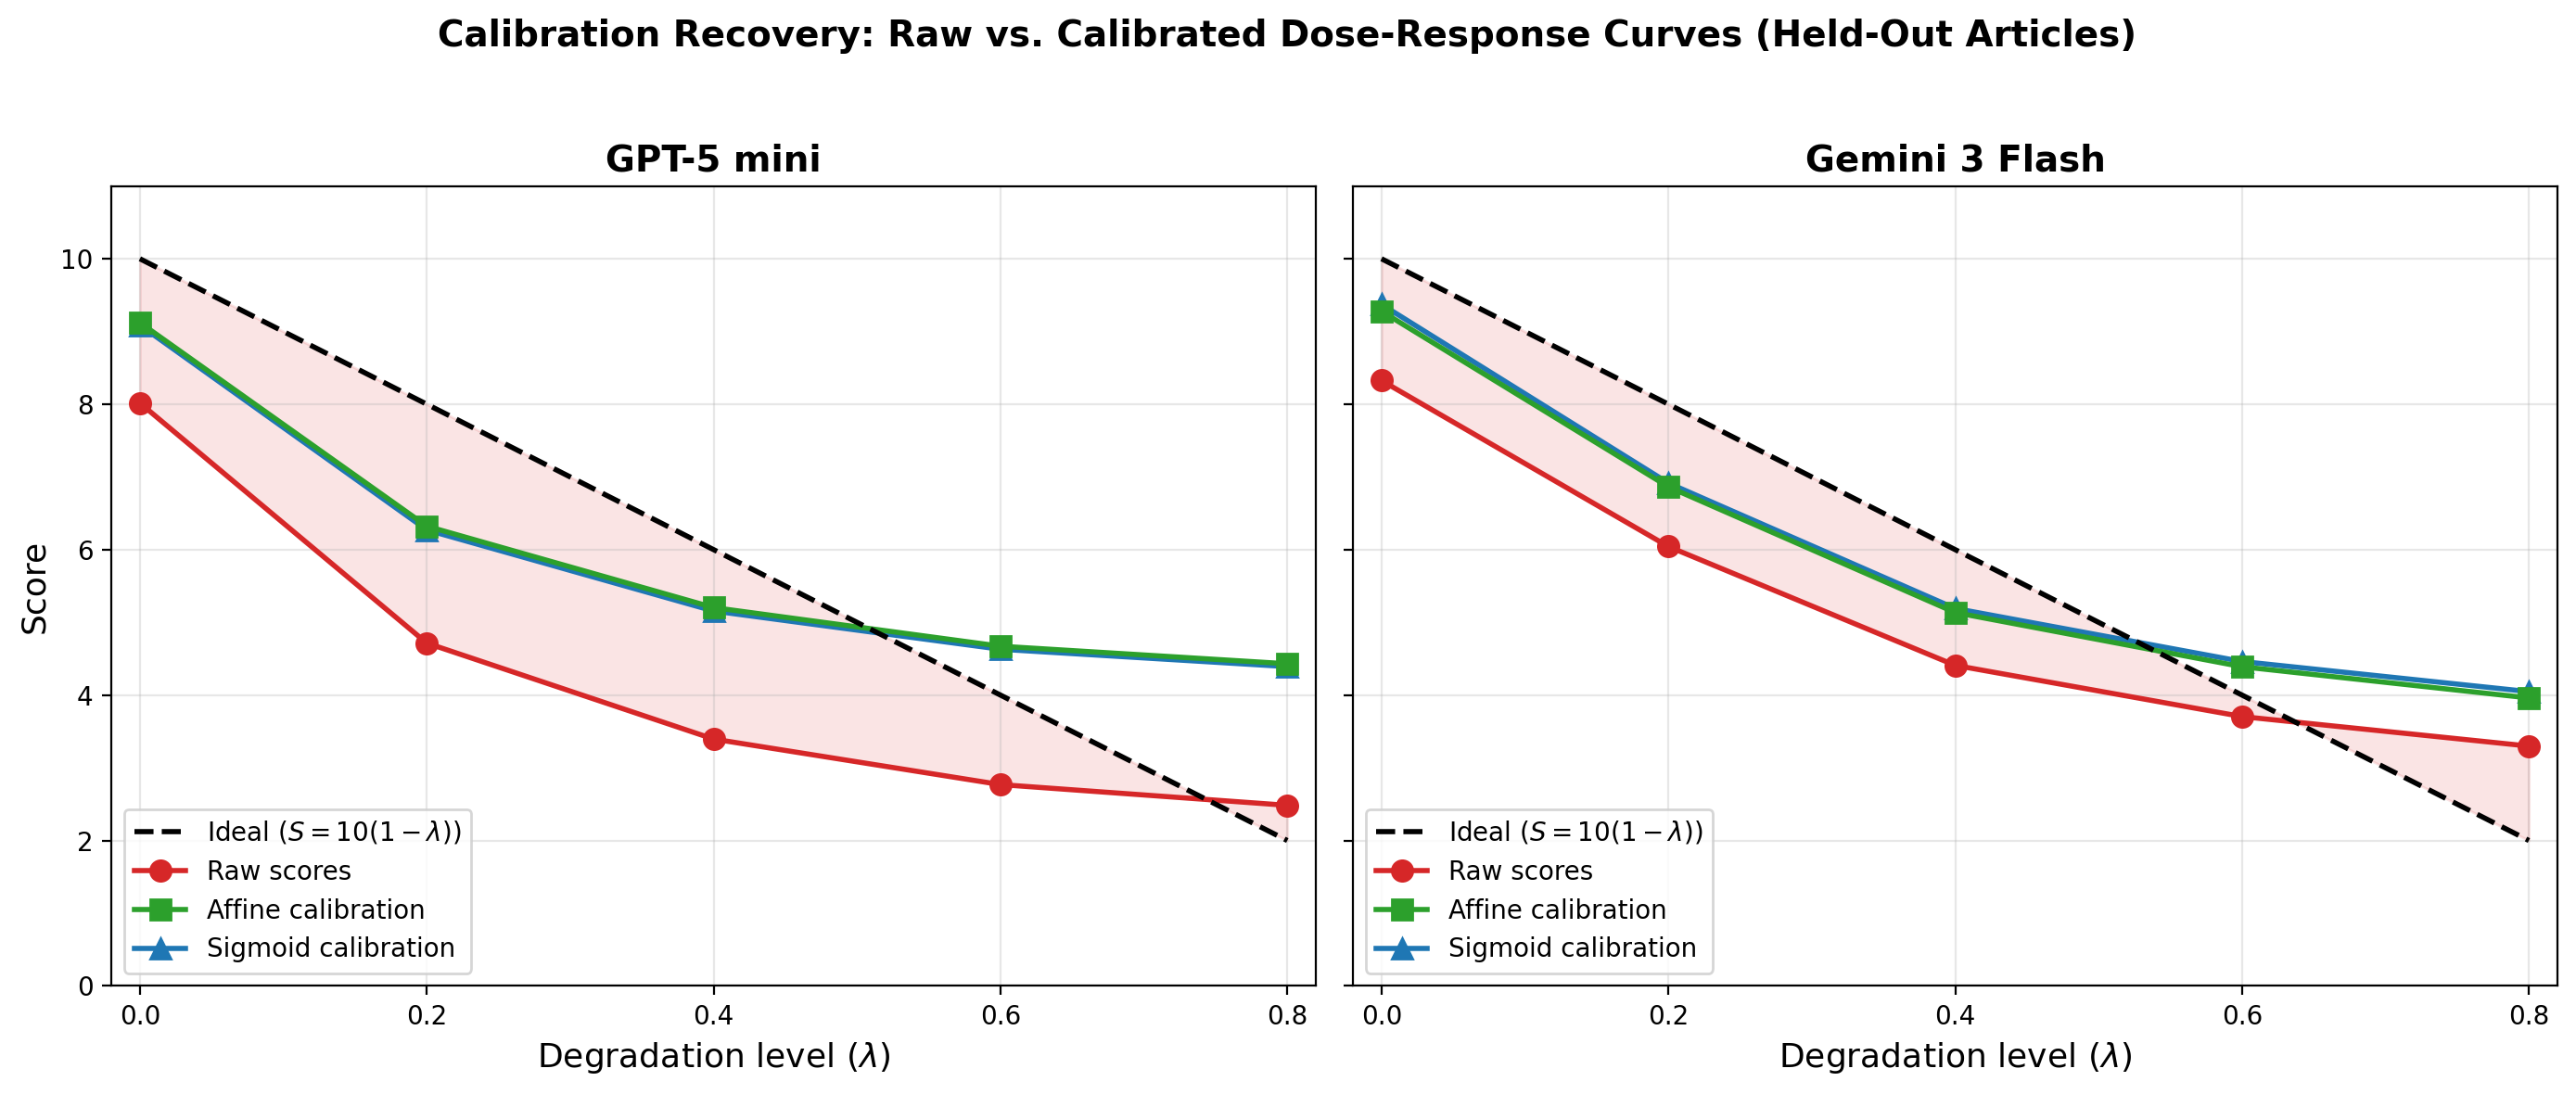
\includegraphics[width=\textwidth]{G15_calibration_recovery.png}
\caption{Dose-response curves before and after calibration, against the ideal reference line (dashed black). Affine, sigmoid, and isotonic (nonparametric) calibrations all converge to nearly identical curves, confirming that the compression is approximately linear and the residual error represents irreducible rank-order noise.}
\label{fig:calibrecovery}
\end{figure}

These results carry a dual message. On the one hand, a simple two-parameter affine correction---requiring only a modest calibration set---recovers a meaningful fraction of the lost accuracy, making post-hoc calibration a practical and low-cost mitigation strategy. On the other hand, the fact that no calibration method (including the nonparametric isotonic upper bound) can reduce RMSE below $\sim$1.6 confirms that compression is not purely an offset problem: the models genuinely fail to spread scores across the full range, losing discriminative information that cannot be recovered by rescaling.

\subsection{Intra-Condition Reliability}

Intraclass correlation coefficients (ICC(1,1)) computed across the three repetitions per condition indicate high scoring consistency across all eleven models (Table~\ref{tab:icc}). The two primary models achieve the highest reliability: overall ICC $= 0.926$ for GPT-5~mini and $0.905$ for Gemini~3~Flash. Most models achieve ICC $> 0.70$, with the notable exception of MiniMax~M2P1 (ICC $= 0.433$), which exhibits substantially higher scoring variability---likely due to its API-based access with potential load-dependent behavior. Grammar consistently elicits the most reliable scoring across models, while coherence shows the most variability.

\begin{figure}[t]
\centering
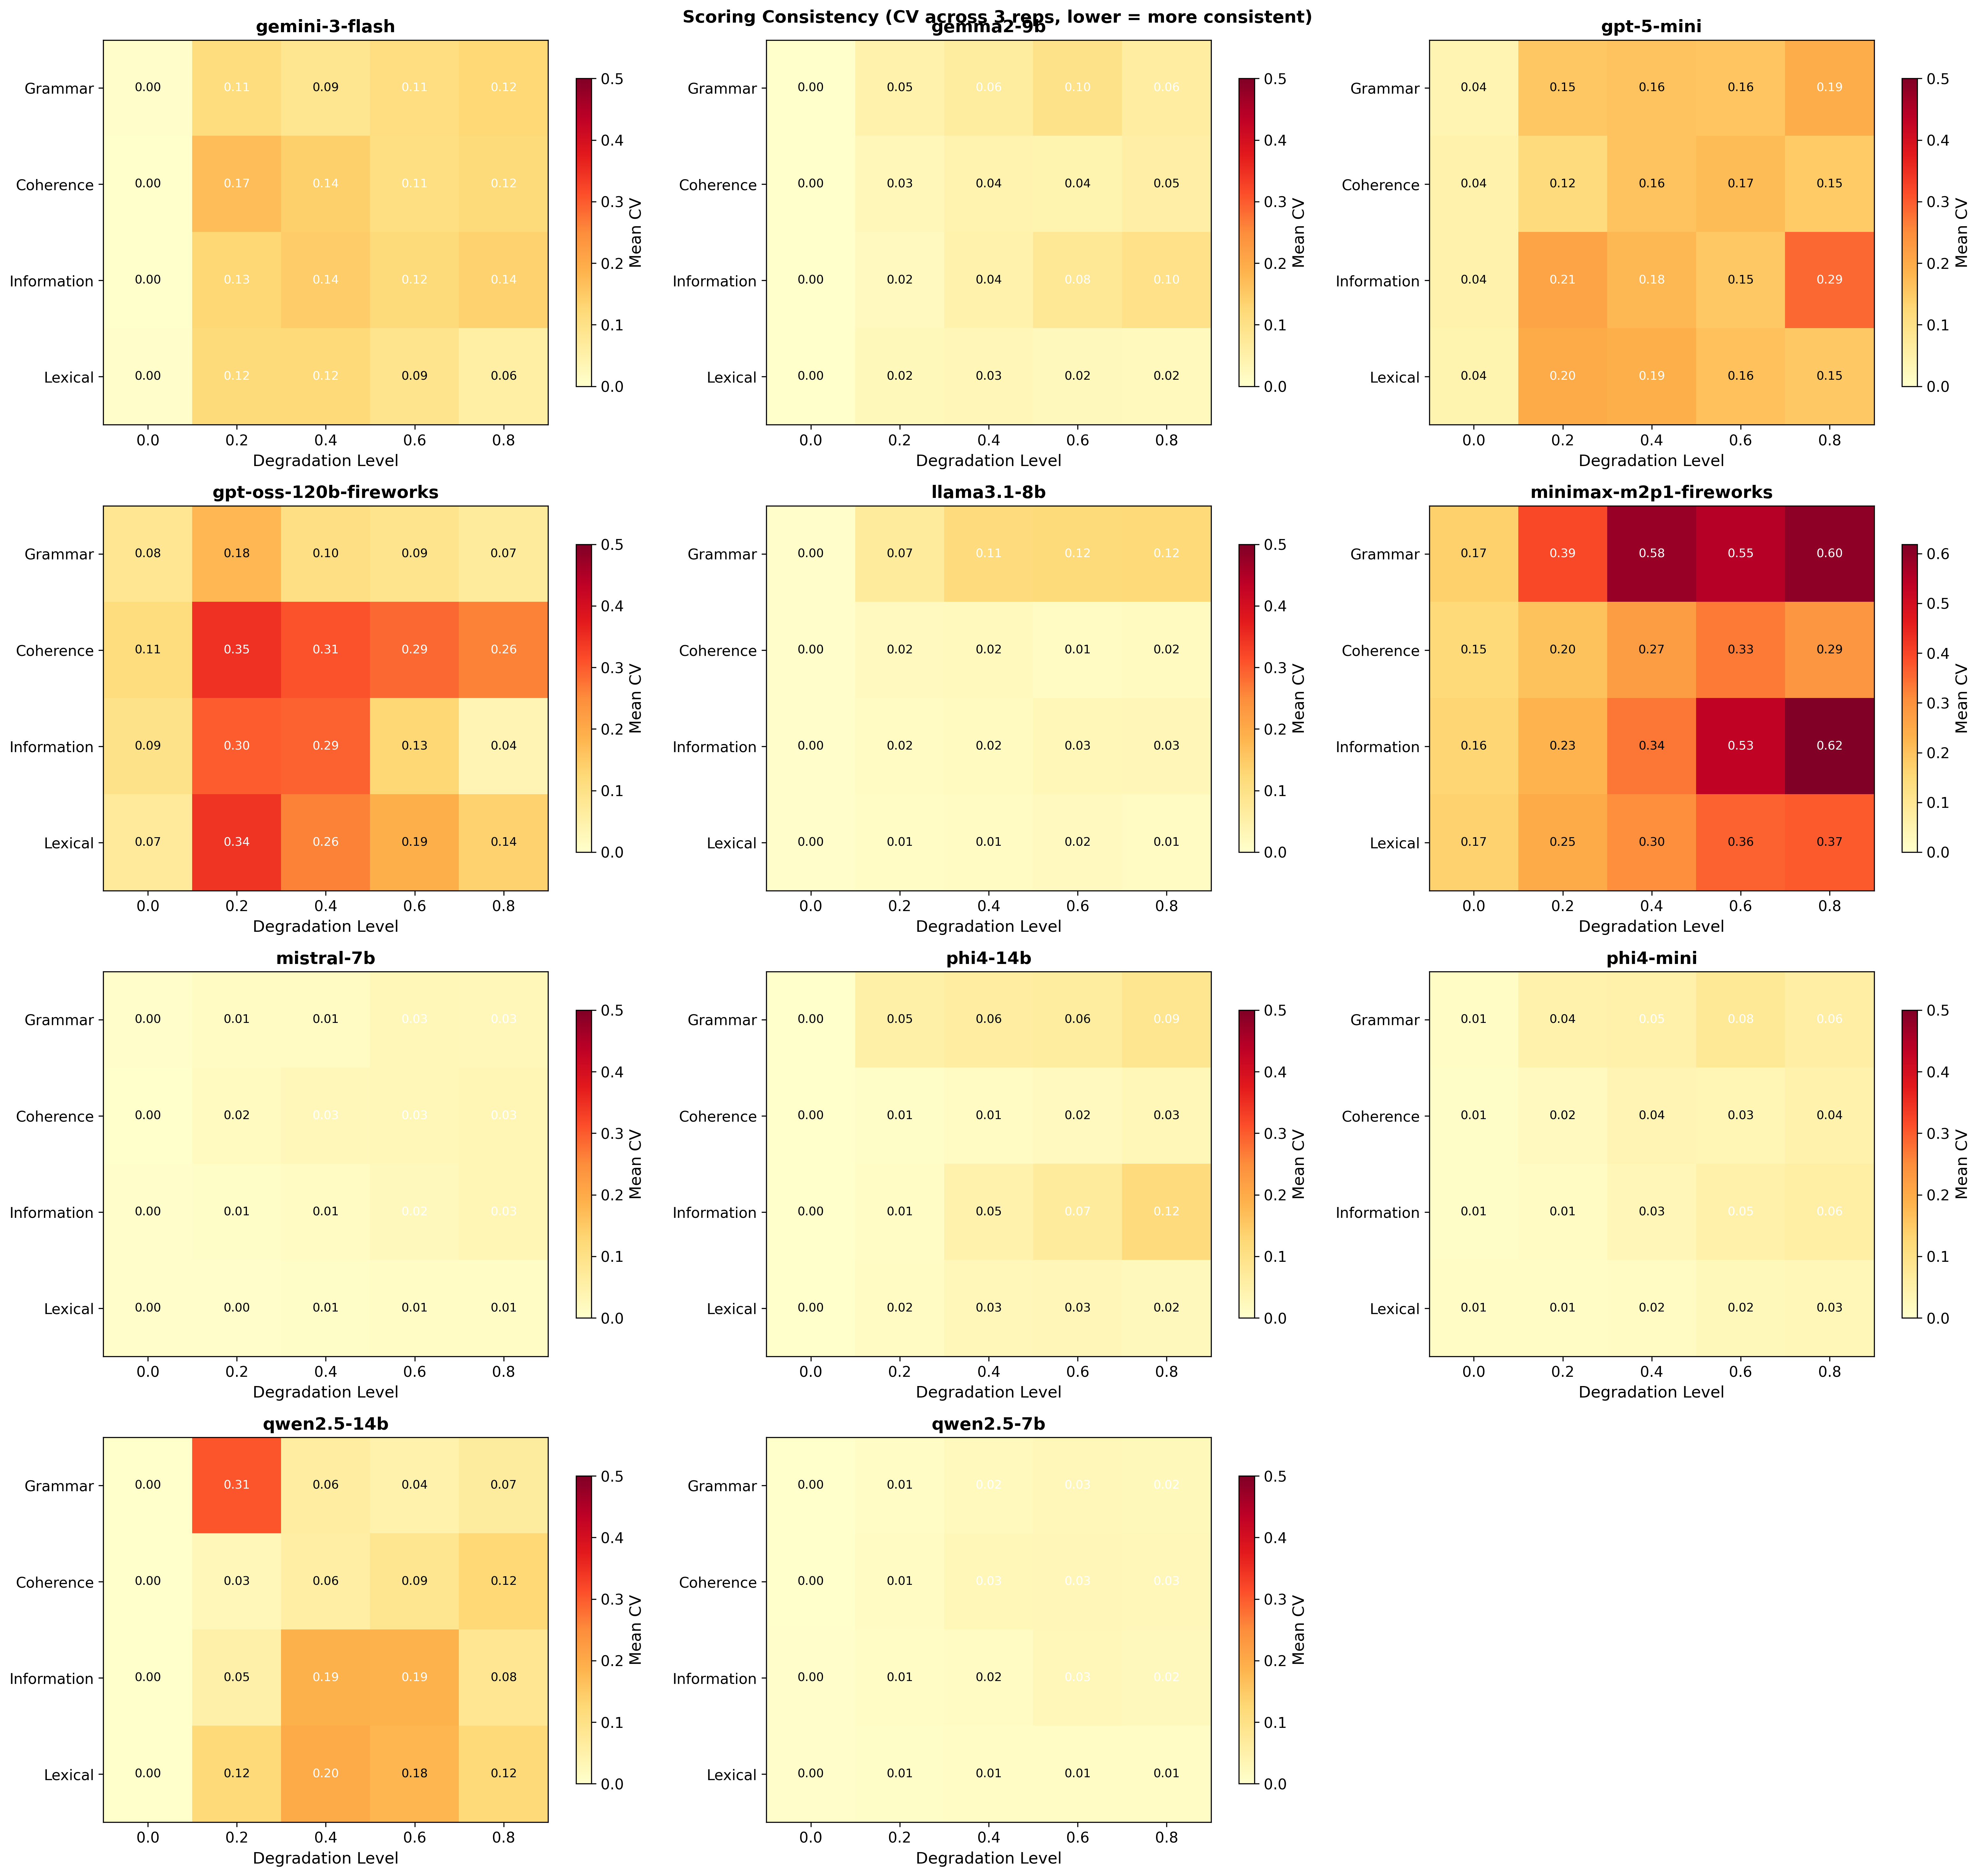
\includegraphics[width=\textwidth]{G12_rep_consistency.png}
\caption{Scoring consistency heatmap: mean coefficient of variation (CV) across three repetitions, by axis and degradation level. Lower values (lighter) indicate more consistent scoring.}
\label{fig:consistency}
\end{figure}

\begin{table}[H]
\centering
\caption{Intra-condition reliability (ICC(1,1)) by axis for all eleven models.}
\label{tab:icc}
\small
\begin{tabular}{@{}lccccc@{}}
\toprule
\textbf{Model} & \textbf{Grammar} & \textbf{Coherence} & \textbf{Info} & \textbf{Lexical} & \textbf{Overall} \\
\midrule
GPT-5 mini & 0.963 & 0.850 & 0.925 & 0.897 & \textbf{0.926} \\
Gemini 3 Flash & 0.950 & 0.844 & 0.913 & 0.890 & \textbf{0.905} \\
Gemma 2 9B & 0.891 & 0.823 & 0.852 & 0.873 & 0.888 \\
Qwen 2.5 14B & 0.845 & 0.605 & 0.856 & 0.744 & 0.849 \\
Phi-4 14B & 0.765 & 0.702 & 0.811 & 0.794 & 0.826 \\
Llama 3.1 8B & 0.716 & 0.689 & 0.711 & 0.767 & 0.805 \\
GPT-OSS 120B & 0.914 & 0.566 & 0.777 & 0.718 & 0.751 \\
Mistral 7B & 0.717 & 0.663 & 0.726 & 0.880 & 0.745 \\
Qwen 2.5 7B & 0.722 & 0.612 & 0.740 & 0.807 & 0.722 \\
Phi-4 mini & 0.619 & 0.734 & 0.759 & 0.778 & 0.719 \\
MiniMax M2P1 & 0.394 & 0.181 & 0.422 & 0.359 & 0.433 \\
\bottomrule
\end{tabular}
\end{table}

\subsection{Effect Sizes}

Within-model effect sizes for the undegraded-vs.-maximally-degraded contrast are extremely large: Cliff's $\delta = 0.986$ (GPT) and $0.984$ (Gemini), with Cohen's $d = 4.65$ and $5.33$ respectively. Between-model effect sizes (Gemini $-$ GPT) are moderate to large across levels, peaking at $\lambda = 0.2$ (Cohen's $d = 0.81$, rank-biserial $r = 0.79$).

\subsection{Covariates and Confounds}

\textbf{Article length.} Adding z-scored article length as a covariate to the mixed model yields a non-significant coefficient for GPT-5~mini ($\beta = -0.058$, $p = 0.21$) but a small, significant coefficient for Gemini~3~Flash ($\beta = -0.151$, $p = 0.002$). Longer articles receive marginally lower scores from Gemini, though the effect size is negligible.

\textbf{Category effects.} Kruskal-Wallis tests on undegraded scores ($\lambda = 0.0$) reveal significant category differences for both models (GPT: $H = 202.6$, $p < 10^{-42}$; Gemini: $H = 377.1$, $p < 10^{-80}$). Both models score Science \& Technology highest (GPT: 8.44; Gemini: 8.73) and Politics \& Society lowest (GPT: 7.58; Gemini: 7.88), as shown in Figure~\ref{fig:category}. This suggests that even among expert-authored articles from a single platform, LLMs exhibit domain-dependent scoring preferences.

\begin{figure}[H]
\centering
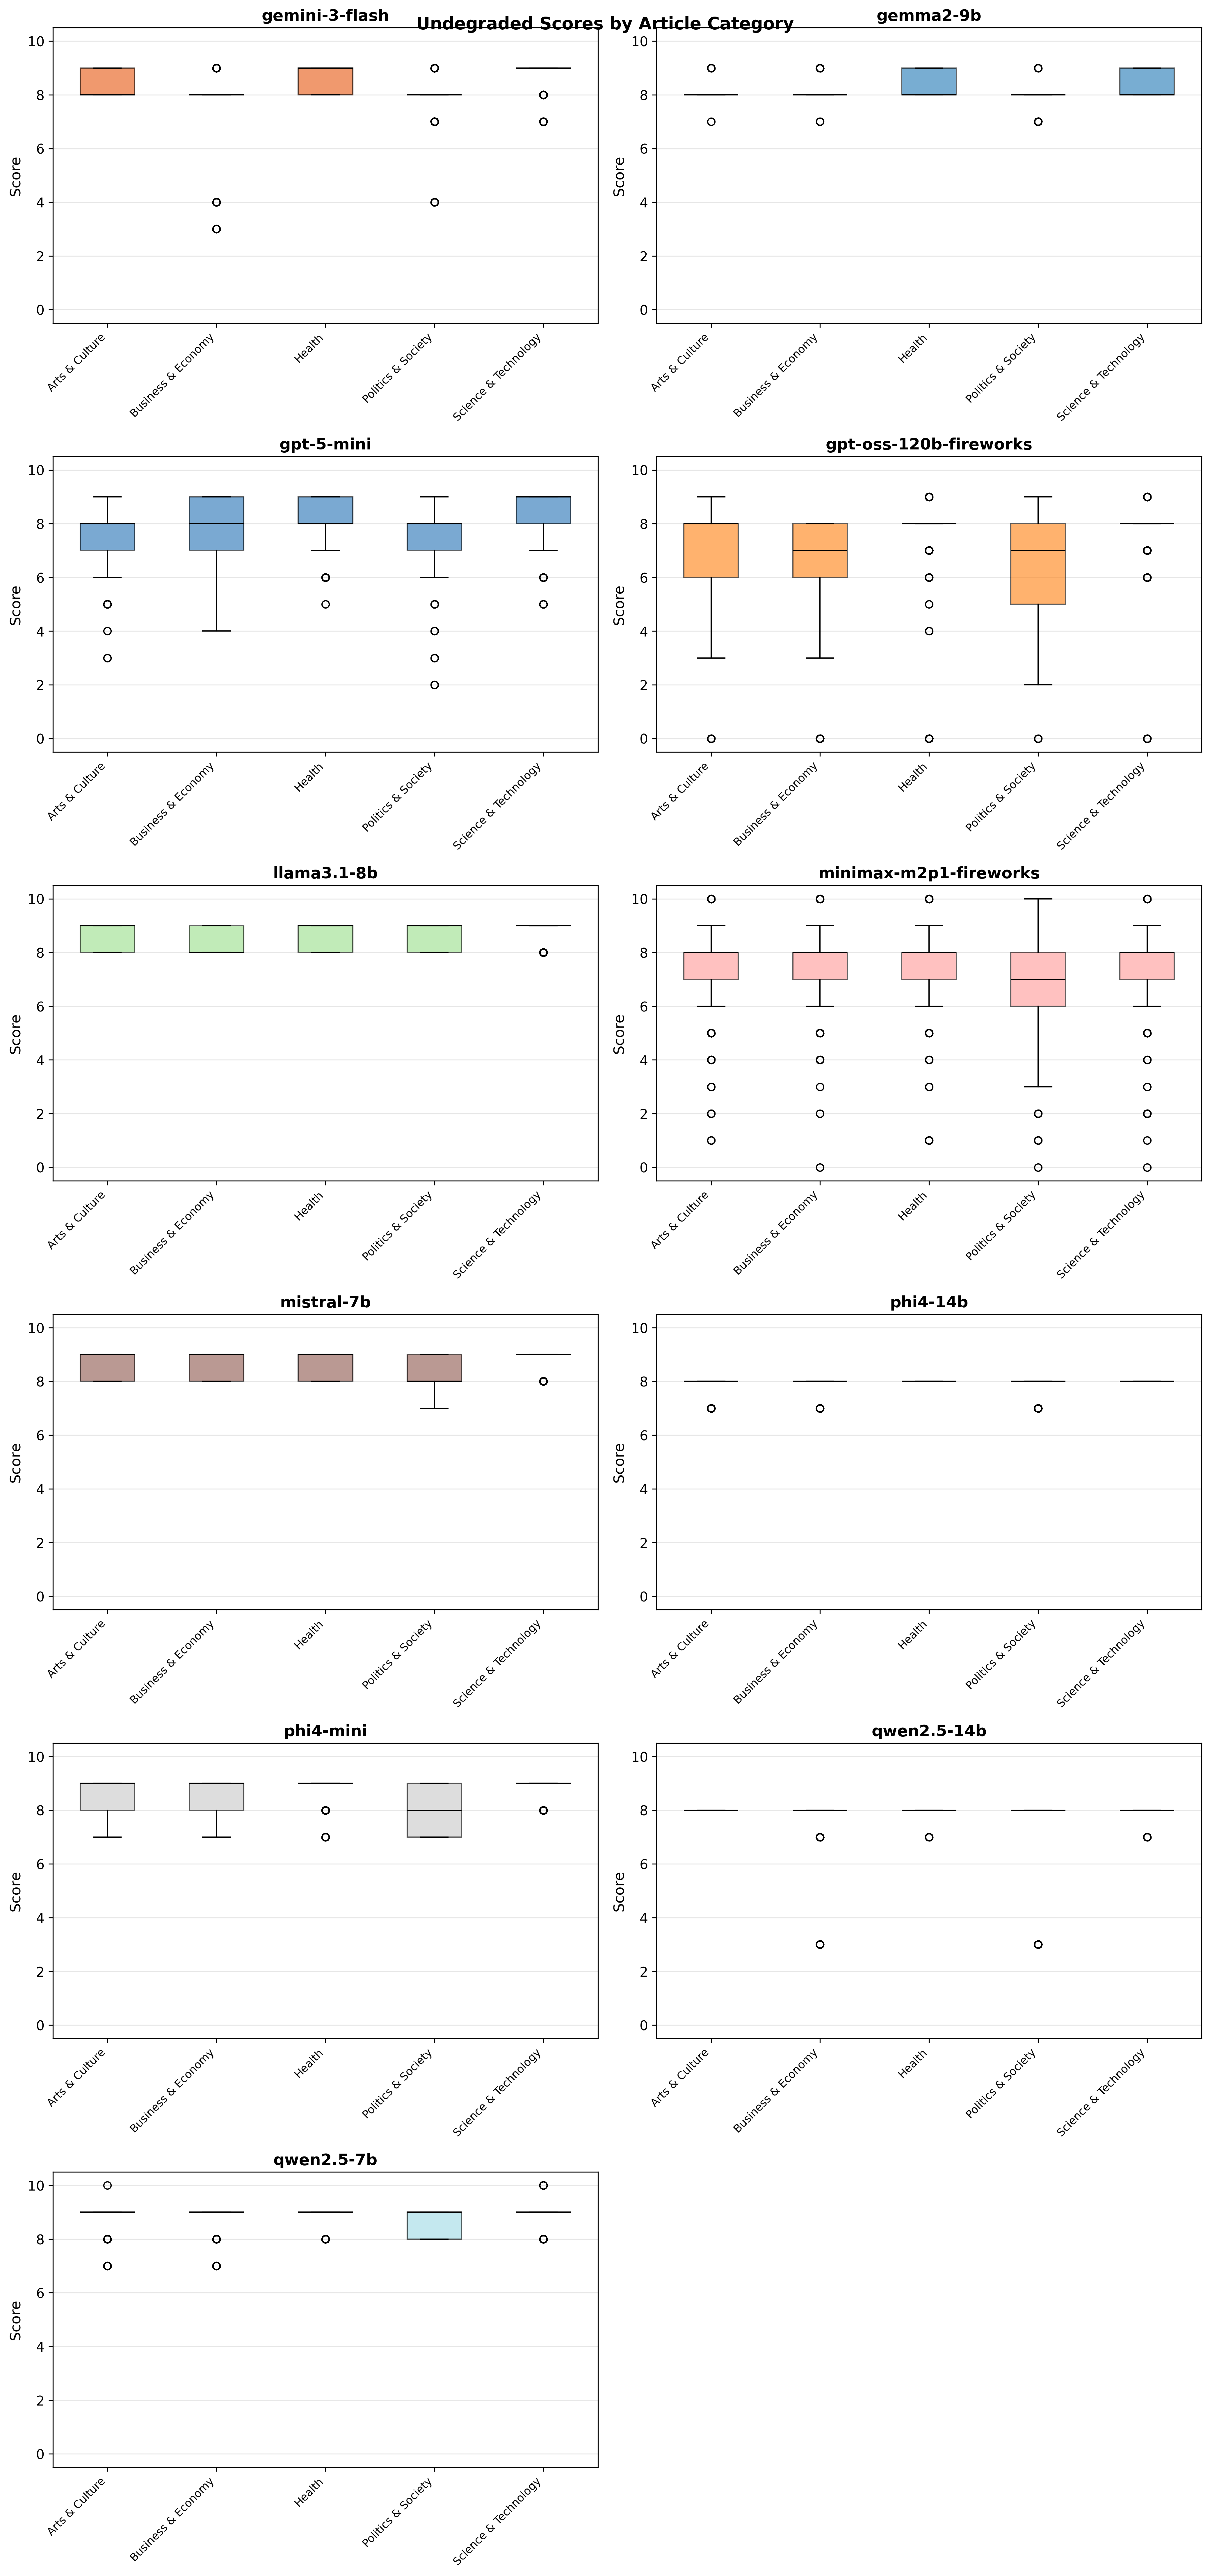
\includegraphics[width=\textwidth,height=0.45\textheight,keepaspectratio]{G13_category_effects.png}
\caption{Undegraded scores ($\lambda = 0.0$) by article category. Both models score Science \& Technology highest and Politics \& Society lowest, despite all articles being expert-authored pieces from The Conversation of comparable editorial quality.}
\label{fig:category}
\end{figure}

\subsection{Multiple Testing Correction}

After Benjamini-Hochberg FDR correction across all 49 $p$-values, 48 remain significant at $\alpha = 0.05$. The sole exception is the article-length covariate for GPT-5~mini ($p_{\text{adj}} = 0.21$).

% ══════════════════════════════════════════════════════════════
% 5. MULTI-MODEL EXTENSION
% ══════════════════════════════════════════════════════════════
\section{Multi-Model Extension}
\label{sec:multimodel}

To assess whether score compression generalizes beyond the two primary models, we replicate the scoring protocol across nine additional models (Table~\ref{tab:models}), ranging from 3.8B parameters (Phi-4~mini) to 228B (MiniMax~M2P1). Each model scores all 9{,}000 samples using the identical minimal prompt. The full results across all eleven models have been reported in Section~\ref{sec:results}; here we focus specifically on the relationship between model size and compression behavior.

\subsection{Compression Across Models}

As shown in Table~\ref{tab:compression}, compression ratios vary widely across the eleven models, from CR $= 0.026$ (Mistral~7B) to CR $= 0.685$ (GPT-5~mini). Smaller models tend to exhibit more extreme compression: models below 10B parameters all achieve CRs below 0.30, while models above 100B all exceed 0.42.

\subsection{Relationship Between Model Size and Compression}

Among the nine models with known parameter counts, there is a positive correlation between $\log_{10}(\text{parameters})$ and compression ratio (Pearson $r = 0.78$, $p = 0.012$). Larger models generally produce more differentiated score distributions. However, this trend is noisy ($n = 9$) and non-monotonic: MiniMax~M2P1 (228B) achieves a lower CR (0.42) than Qwen~2.5~14B (0.45), and Gemma~2~9B achieves a high Spearman $\rho$ (0.70) despite a modest CR (0.30), suggesting that model size alone does not determine compression severity. Architecture, training data, and RLHF procedures likely play important roles.

We note that a correlation on nine data points, while statistically significant, should not be over-interpreted. We characterize this as a \emph{trend} rather than a scaling law; confirmation across a broader model landscape is needed.

% ══════════════════════════════════════════════════════════════
% 6. MITIGATION STRATEGIES
% ══════════════════════════════════════════════════════════════
\section{Mitigation Strategies}
\label{sec:mitigation}

Score compression reduces the discriminative utility of LLM-generated ratings. We evaluate five mitigation strategies, each targeting a different aspect of the problem. Four are post-hoc corrections applied to existing scores; one modifies the scoring prompt itself.

\subsection{Quantile Normalization}

The simplest mitigation: map the empirical score distribution to a target distribution via quantile matching. We test two targets:
\begin{itemize}[nosep]
    \item \textbf{Uniform$[0, 10]$}: Forces scores to span the full range uniformly.
    \item \textbf{Beta$(2, 2)$}: Maps to a symmetric, bell-shaped distribution on $[0, 10]$, avoiding the artificial uniformity of the first target.
\end{itemize}
Because quantile normalization is a monotonic transformation, it preserves rank order: Spearman $\rho$ and pairwise accuracy are unchanged by construction. Only the \emph{distributional shape} (and hence the compression ratio) is affected. This method requires no logprobs and applies to all models.

\subsection{Expected-Score Rescaling}

For models that return token-level log-probabilities over the score tokens (0--10), we replace the argmax score with the probability-weighted expected value:
\begin{equation}
    \hat{S} = \mathbb{E}[S] = \sum_{k=0}^{10} k \cdot p(k)
\end{equation}
where $p(k)$ is the softmax probability of the token representing score $k$. This recovers information from the full probability distribution that argmax discards. This method is available only for the nine models that return logprobs (Table~\ref{tab:models}).

\subsection{Asymmetry Correction}

An extension of expected-score rescaling that corrects for skewness in the score probability distribution:
\begin{equation}
    \hat{S}_{\text{adj}} = \mathbb{E}[S] - \alpha \cdot \text{skewness}(p)
\end{equation}
where $\alpha$ is tuned via five-fold cross-validation (GridSearchCV) to minimize RMSE against the proxy ground truth. In practice, the optimal $\alpha$ was found to be 0.0 for all models, reducing this method to expected-score rescaling.

\subsection{Auxiliary Regression}

A supervised post-hoc approach: train a regressor to predict the proxy ground truth from logprob-derived features. We extract four feature families:
\begin{itemize}[nosep]
    \item \textbf{A1}: entropy, $p_{\text{ceiling}}$ (= $p(9) + p(10)$), expected score, top-2 gap.
    \item \textbf{A2}: A1 + KL divergence from uniform, expected-minus-argmax gap.
    \item \textbf{B}: Full 11-dimensional probability vector $(p_0, \ldots, p_{10})$.
    \item \textbf{C}: A2 + B (all features).
\end{itemize}
Each feature set is paired with two regressors (Ridge, XGBoost), yielding up to eight models per LLM. We use GroupKFold cross-validation (grouping by article) to prevent text leakage and select the best variant per LLM by RMSE. This method is available only for the nine logprob models.

\subsection{Contrastive Anchor Prompting}

A prompt-level intervention: prepend explicit score anchors to the system message (\eg ``A score of 0 means the text is completely unreadable garbage; a score of 10 means the text is flawless, publication-quality prose''). We test this on the two API models (GPT-5~mini and Gemini~3~Flash) using 200 randomly selected samples, comparing the anchor prompt against the standard minimal prompt. This is the only mitigation that modifies the scoring protocol itself rather than post-processing scores.

% ══════════════════════════════════════════════════════════════
% 7. MITIGATION RESULTS
% ══════════════════════════════════════════════════════════════
\section{Mitigation Results}
\label{sec:mitresults}

Because different methods apply to different model subsets (Table~\ref{tab:models}), na\"ive averaging across all available models would create an apples-to-oranges comparison. We therefore report controlled comparisons on matching model sets.

\subsection{Controlled Comparisons}

Table~\ref{tab:mitcompare} reports mean metrics across the nine logprob models, where all post-hoc methods can be evaluated on the same population.

\begin{table}[t]
\centering
\caption{Mitigation comparison on the nine logprob models. All methods are evaluated on the same nine models for a fair comparison. Spearman $\rho$ and pairwise accuracy (PA) are computed against proxy ground truth. CR here is the range-based compression ratio $(\max - \min)/10$, which measures how much of the 0--10 scale is utilized. $\Delta\rho$ is the change from raw baseline.}
\label{tab:mitcompare}
\begin{tabular}{@{}lcccc@{}}
\toprule
\textbf{Method} & \textbf{Spearman} $\rho$ & $\Delta\rho$ & \textbf{CR} & \textbf{PA} \\
\midrule
Raw (baseline) & 0.458 & --- & 0.689 & 0.518 \\
Quantile (uniform) & 0.458 & 0.000 & 0.922 & 0.518 \\
Quantile (Beta) & 0.458 & 0.000 & 0.847 & 0.518 \\
Expected score $\mathbb{E}[S]$ & 0.490 & +0.032 & 0.579 & 0.649 \\
Asymmetry fix ($\alpha = 0$) & 0.490 & +0.032 & 0.579 & 0.649 \\
Auxiliary regressor (best) & 0.496 & +0.038 & 0.919 & 0.702 \\
\bottomrule
\end{tabular}
\end{table}

Several findings emerge:

\begin{enumerate}[nosep]
    \item \textbf{Quantile normalization preserves rank order exactly.} By construction, Spearman $\rho$ and pairwise accuracy are unchanged---quantile mapping is a monotonic transformation. However, it dramatically expands the compression ratio from 0.689 to 0.922 (uniform target), recovering most of the lost range.
    \item \textbf{Expected-score rescaling provides modest rank improvement.} Replacing the argmax with $\mathbb{E}[S]$ improves mean Spearman $\rho$ from 0.458 to 0.490 and pairwise accuracy from 0.518 to 0.649, indicating that the full probability distribution contains quality-relevant information that argmax discards.
    \item \textbf{Asymmetry correction reduces to expected-score rescaling.} The optimal $\alpha$ was 0.0 for all nine models, indicating negligible skewness-driven bias. This suggests that the primary benefit of logprob-based rescaling comes from using the full distribution, not from correcting its shape.
    \item \textbf{Auxiliary regression offers the best rank improvement.} The best per-model regressor improves mean $\rho$ to 0.496 and pairwise accuracy to 0.702 while also achieving a high CR of 0.919. However, this method requires supervised training on proxy ground truth and is therefore less practical than unsupervised alternatives.
    \item \textbf{No method dramatically changes rank correlation.} The largest $\rho$ improvement is $+0.038$ (auxiliary regression), suggesting that the models' rank-order information is largely baked into their argmax scores and cannot be substantially recovered post hoc.
\end{enumerate}

\subsection{Contrastive Anchor Prompting}

On the two API models, contrastive prompting yields mixed results (Table~\ref{tab:contrastive}). Gemini~3~Flash shows a small improvement ($\rho: 0.801 \to 0.836$), while GPT-5~mini shows a meaningful degradation ($\rho: 0.729 \to 0.619$). The mean raw $\rho$ on these two models is 0.765; after contrastive prompting, it drops to 0.727. Compression ratios are unchanged.

\begin{table}[t]
\centering
\caption{Contrastive anchor prompting on API models ($n = 200$ samples per model). $\rho$ is Spearman correlation against proxy ground truth.}
\label{tab:contrastive}
\begin{tabular}{@{}lccc@{}}
\toprule
\textbf{Model} & \textbf{Raw} $\rho$ & \textbf{Contrastive} $\rho$ & $\Delta\rho$ \\
\midrule
Gemini 3 Flash & 0.801 & 0.836 & $+$0.035 \\
GPT-5 mini & 0.729 & 0.619 & $-$0.110 \\
\midrule
\textbf{Mean} & 0.765 & 0.727 & $-$0.038 \\
\bottomrule
\end{tabular}
\end{table}

The failure of contrastive prompting for GPT-5~mini may reflect the reasoning model's tendency to overthink anchor instructions, producing more variable and less calibrated scores. For Gemini, the explicit anchors appear to provide useful calibration guidance. Given the small sample ($n = 2$ models, 200 samples each), we refrain from strong conclusions about the general efficacy of prompt-level interventions.

\subsection{Per-Model Breakdown}

Figure~\ref{fig:spearman_bar} shows per-model Spearman $\rho$ across all methods. The benefit of logprob-based methods varies substantially by model. For high-performing models (\eg Gemma~2~9B, GPT-OSS~120B), expected-score rescaling provides meaningful improvement. For low-performing models (\eg Mistral~7B, $\rho_{\text{raw}} = 0.138$), auxiliary regression produces negative $\rho$ ($-0.112$), indicating that logprob features are not predictive of quality when the base model fails to discriminate degradation levels. This highlights a fundamental limitation: post-hoc corrections cannot rescue a model that lacks the underlying quality signal.

\begin{figure}[H]
\centering
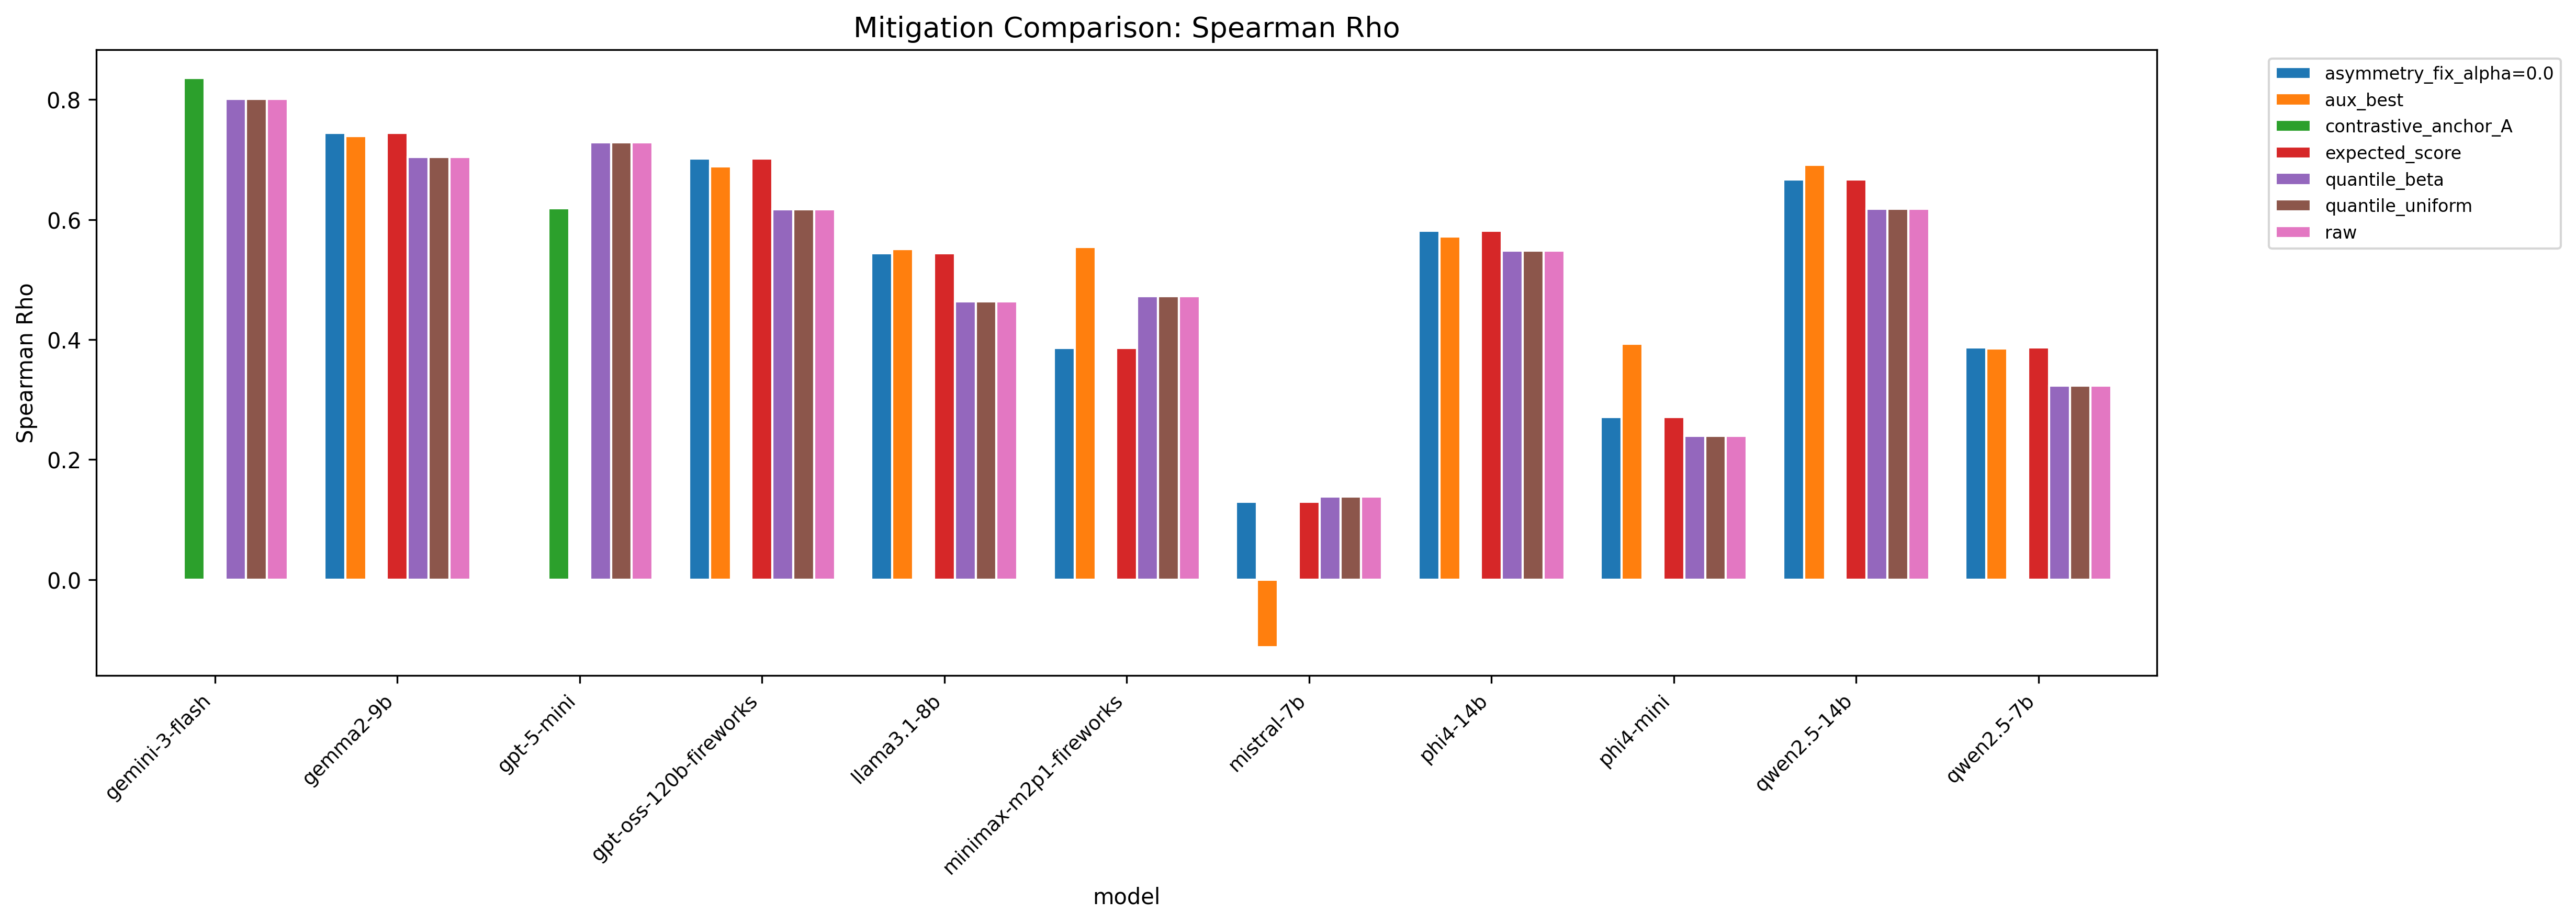
\includegraphics[width=\textwidth]{spearman_rho_barplot.png}
\caption{Spearman $\rho$ against proxy ground truth for each model and mitigation method. Logprob-based methods (E[$S$], auxiliary regression) are available only for the nine models with logprob access.}
\label{fig:spearman_bar}
\end{figure}

% ══════════════════════════════════════════════════════════════
% 8. DISCUSSION
% ══════════════════════════════════════════════════════════════
\section{Discussion}
\label{sec:discussion}

\subsection{The Compression Effect}

Our results demonstrate that score compression is a robust, reproducible phenomenon across all eleven models tested. In the primary two-model study, both GPT-5~mini and Gemini~3~Flash compress the effective scoring range to 62--69\% of the ideal, with neither model ever producing the minimum (0) or maximum (10) score on a 0--10 scale. Across all eleven models and approximately 99{,}000 total evaluations, compression ratios range from 0.02 to 0.69. This is not an artifact of the experimental design: calibrated simulations show that a simple linear scorer with equivalent noise would produce hundreds of extreme scores.

The compression manifests asymmetrically. At the ceiling, pristine texts receive mean scores of 7.3--8.7 across models rather than the expected 10 (Figure~\ref{fig:undegraded}). At the floor, maximally degraded texts receive mean scores well above the expected minimum. The net effect is a concave dose-response curve, confirmed by significant quadratic terms in 32 of 44 axis$\times$model regressions. The residual diagnostics (Figure~\ref{fig:residuals}) further confirm the non-linear relationship.

\begin{figure}[H]
\centering
\includegraphics[width=\textwidth,height=0.45\textheight,keepaspectratio]{G14_residuals.png}
\caption{Residual diagnostics from linear regression of score on degradation level. Left: residuals vs.\ fitted values with LOWESS smoother (red), showing systematic curvature. Right: Q-Q plots showing heavy-tailed, discrete residuals---expected for bounded integer scores.}
\label{fig:residuals}
\end{figure}

\subsection{Linearity as Approximation}

Our primary analysis relies on a linear reference model $S = 10(1 - \lambda)$ to quantify compression. While this provides an interpretable and assumption-lean benchmark, the empirical dose-response relationship is not perfectly linear. Nested $F$-tests reveal highly significant quadratic terms in all eight axis$\times$model regressions (Table~\ref{tab:nonlin}), and the dose-response curves (Figure~\ref{fig:doseresponse}) are visibly concave: sensitivity is highest at low degradation levels and diminishes as quality approaches the floor. This is consistent with psychophysical diminishing returns---the perceptual difference between a pristine and a mildly degraded text is larger than the difference between a moderately and a severely degraded text.

Critically, the choice of a linear reference does not undermine our core findings. First, the complete absence of boundary scores (0 and 10 in six of eleven models, across approximately 54{,}000 evaluations) is a model-free observation that requires no reference function. Second, the calibration recovery experiment (Section~\ref{sec:calibration}) shows that affine, sigmoid, and isotonic calibrations all converge to nearly identical curves, indicating that the residual non-linearity beyond an affine correction is modest. Third, a concave ground-truth function would imply that our linear reference \emph{understates} the true compression, making our reported compression ratios conservative. We therefore retain the linear model as a deliberate analytical choice---it is the simplest reference that permits closed-form compression ratios while erring on the side of underestimating the effect.

\subsection{Axis-Specific Sensitivity}

The models agree on the relative ordering of axis sensitivity: across all eleven models, information deletion consistently elicits the steepest response while coherence disruption elicits the shallowest (Table~\ref{tab:slopes}). This ordering---information $>$ grammar $>$ lexical $>$ coherence---holds for the top-performing models, though the magnitude varies dramatically (mean slopes from $-6.46$ to $-0.28$). The significant three-way interactions in the mixed model confirm that the two primary models weight these dimensions differently.

The low sensitivity to coherence disruption is particularly noteworthy. Shuffling sentences destroys argumentative flow and coreference chains while preserving all surface-level features (grammar, vocabulary, factual content). The models' relative insensitivity suggests they may weight local, sentence-level quality features more heavily than global discourse structure.

\subsection{Systematic Inter-Model Bias}

Despite high agreement ($r = 0.84$), Gemini~3~Flash scores one point higher than GPT-5~mini on the same texts. This is a \emph{systematic} offset, not random noise: rank-biserial $r = 0.71$ indicates that Gemini scores higher on 85\% of disagreement pairs. The offset is smallest on coherence (median difference = 0) and largest on grammar, information, and lexical axes (median difference = +1 each).

This finding has practical implications: scores from different LLM providers are not interchangeable. A threshold calibrated on GPT scores would systematically fail if applied to Gemini scores, and vice versa.

\subsection{Reliability}

Both primary models achieve excellent intra-condition reliability (ICC $> 0.90$), and ten of eleven models achieve ICC $> 0.70$ (Table~\ref{tab:icc}). This confirms that compression is not a noise phenomenon---it is a stable, deterministic property of the scoring function.

\subsection{Implications}

These findings carry several practical implications:

\begin{enumerate}[nosep]
    \item \textbf{Score calibration is necessary.} Raw LLM scores should not be treated as ground truth on the nominal scale. Quantile normalization is a simple, effective, and model-agnostic approach to recover the lost range.
    \item \textbf{Model-specific thresholds.} Applications using score thresholds must calibrate per model. A ``good'' score of 7 from GPT-5~mini is not equivalent to a 7 from Gemini~3~Flash.
    \item \textbf{Ordinal, not interval.} LLM scores should be treated as ordinal rather than interval data. The spacing between adjacent scores is not uniform, and the scale has effective rather than nominal endpoints.
    \item \textbf{Axis awareness.} Compression severity varies by quality dimension. Users seeking to evaluate coherence should be aware that LLMs may be less sensitive to discourse-level quality variation.
    \item \textbf{Post-hoc corrections help modestly.} Our mitigation experiments show that quantile normalization recovers distributional range, expected-score rescaling provides modest rank improvements, and auxiliary regression offers the best gains where logprobs are available. However, the largest rank improvement observed ($\Delta\rho = +0.038$) is small, indicating that the models' quality rankings are largely determined at inference time and cannot be substantially altered post hoc.
    \item \textbf{Prompt-level interventions are unreliable.} Contrastive anchor prompting produced inconsistent results across two models, suggesting that prompt engineering alone is not a robust mitigation strategy for score compression.
    \item \textbf{Model scale matters.} Larger models generally exhibit less extreme compression (higher CRs), but the relationship is noisy and exceptions exist. Users should not assume that a larger model will automatically produce better-calibrated scores.
\end{enumerate}

\subsection{Limitations}

Several limitations warrant acknowledgment. First, our degradation axes, while designed to be orthogonal, may have residual correlations (\eg information deletion may incidentally affect coherence). Second, the corpus is limited to English-language expository text from a single source; generalization to other languages, genres, or domains requires further investigation. Third, while we evaluate eleven models---a substantial improvement over the initial two---the effect may vary further across the broader model landscape, particularly for commercial models that do not expose log-probabilities.

Fourth, the temperature asymmetry between the two primary models (GPT-5~mini at 1.0 vs.\ Gemini~3~Flash at 0.0) is a meaningful confound. Higher temperatures flatten the output probability distribution over tokens, which could theoretically push the model away from extreme scores and toward the center of the scale---raising the question of whether GPT-5~mini's compression is an artifact of its sampling temperature rather than an intrinsic scoring bias. However, this hypothesis predicts that GPT (at $T = 1.0$) should exhibit \emph{greater} compression than Gemini (at $T = 0.0$). In fact, the opposite is observed: GPT achieves a compression ratio of 0.685 vs.\ 0.621 for Gemini, meaning the model with deterministic decoding compresses \emph{more}. This directional mismatch provides evidence against a temperature-driven explanation. Additionally, our ICC analysis shows that GPT's intra-condition reliability remains excellent (ICC $= 0.926$) despite the higher temperature, suggesting that the reasoning model's internal deliberation stabilizes outputs even at temperature~1.0. A majority-vote aggregation across the three repetitions per condition yields near-identical mean scores (mean absolute difference from raw mean $< 0.05$), indicating that the stochasticity does not meaningfully shift point estimates. Nevertheless, future work should compare models at matched temperature settings where API constraints permit.

Fifth, our mitigation comparison is constrained by data availability: logprob-based methods (expected score, auxiliary regression) can only be evaluated on the nine models that return token-level probabilities, while contrastive prompting was tested on only two API models. We address this by reporting controlled comparisons on matching model sets (Table~\ref{tab:mitcompare}) rather than na\"ively averaging across unequal populations.

Sixth, our ideal calibration reference line $S = 10(1 - \lambda)$ assumes that text quality degrades linearly with the corruption parameter. In practice, human perception of quality may be non-linear---for instance, removing 80\% of content words may render text effectively worthless ($S \approx 0$) rather than quality-2. We emphasize that this reference is a mathematical construct chosen for interpretability, not a claim about perceptual scaling. Crucially, our strongest finding---that six of eleven models never assign a score of 0 or 10 across 9{,}000 samples each, despite calibrated simulations predicting hundreds---is entirely independent of the linearity assumption. The compression ratio would, if anything, be \emph{understated} under a concave ground-truth function, making our linear reference a conservative benchmark.

Seventh, our scoring prompt is intentionally minimal to measure intrinsic calibration bias. Because LLM outputs are sensitive to system instructions, a reviewer might ask whether the distributional bias disappears under a strict grading rubric or few-shot examples that explicitly anchor scores of 0 and 10. Our contrastive anchor experiment (Section~\ref{sec:mitresults}) provides a partial answer: explicit anchors produced inconsistent effects across two models, suggesting that the bias is not purely a prompt-level phenomenon. However, more elaborate prompt designs---including chain-of-thought reasoning, decomposed evaluation, or fine-grained rubrics---remain untested and may yield different results.

% ══════════════════════════════════════════════════════════════
% 6. CONCLUSION
% ══════════════════════════════════════════════════════════════
\section{Conclusion}
\label{sec:conclusion}

We have demonstrated that score compression is a robust, reproducible phenomenon across eleven language models spanning 3.8B to 228B parameters and multiple providers, confirmed through approximately 99{,}000 total evaluations. In a detailed two-model study, both GPT-5~mini and Gemini~3~Flash systematically avoid the extremes of the 0--10 scale, compressing the effective range to 62--69\% of the ideal. In a broader eleven-model extension, compression ratios range from 0.02 to 0.69, correlating positively with model size ($r = 0.78$) but with notable exceptions.

Five mitigation strategies yield a nuanced picture: quantile normalization efficiently recovers distributional range, logprob-based rescaling modestly improves rank correlation, auxiliary regression provides the best pairwise accuracy gains, and contrastive anchor prompting produces inconsistent results. The largest rank-correlation improvement is $+0.038$, indicating that the models' quality rankings are largely baked into their inference-time outputs and cannot be substantially altered post hoc.

The title of this paper reflects the core finding: no one gets an A---LLMs resist assigning top marks just as they resist failing grades, funneling their evaluations into a safe middle range. As LLMs are increasingly relied upon for automated text evaluation, understanding and correcting this distributional bias is essential for maintaining evaluation fidelity.

\subsection*{Reproducibility}

The complete codebase, including the degradation engine, scoring scripts, analysis pipeline, and all raw score data, is publicly available at \url{https://github.com/idreesaziz/Distributional-Bias-in-LLM-Text-Scoring}. All experiments are deterministically reproducible via MD5-seeded randomness.

% ══════════════════════════════════════════════════════════════
% REFERENCES
% ══════════════════════════════════════════════════════════════
\begin{thebibliography}{9}

\bibitem[Guilford(1954)]{guilford1954psychometric}
Guilford, J.~P. (1954).
\newblock \emph{Psychometric Methods}.
\newblock McGraw-Hill, New York, 2nd edition.

\bibitem[Ke \& Ng(2019)]{ke2019automated}
Ke, Z. and Ng, V. (2019).
\newblock Automated essay scoring: A survey of the state of the art.
\newblock In \emph{Proceedings of the 28th International Joint Conference on Artificial Intelligence}, pages 6300--6308.

\bibitem[Kocmi \& Federmann(2023)]{kocmi2023large}
Kocmi, T. and Federmann, C. (2023).
\newblock Large language models are state-of-the-art evaluators of translation quality.
\newblock In \emph{Proceedings of the 24th Annual Conference of the European Association for Machine Translation}, pages 193--203.

\bibitem[Liu et~al.(2023)]{liu2023geval}
Liu, Y., Iter, D., Xu, Y., Wang, S., Xu, R., and Zhu, C. (2023).
\newblock G-Eval: {NLG} evaluation using {GPT-4} with better human alignment.
\newblock In \emph{Proceedings of the 2023 Conference on Empirical Methods in Natural Language Processing}, pages 2511--2522.

\bibitem[Stevens(1971)]{stevens1971issues}
Stevens, S.~S. (1971).
\newblock Issues in psychophysical measurement.
\newblock \emph{Psychological Review}, 78(5):426--450.

\bibitem[Wang et~al.(2023)]{wang2023large}
Wang, P., Li, L., Chen, L., Zhu, D., Lin, B., Cao, Y., Liu, Q., Liu, T., and Sui, Z. (2023).
\newblock Large language models are not fair evaluators.
\newblock \emph{arXiv preprint arXiv:2305.17926}.

\bibitem[Zheng et~al.(2023)]{zheng2023judging}
Zheng, L., Chiang, W.-L., Sheng, Y., Zhuang, S., Wu, Z., Zhuang, Y., Lin, Z., Li, Z., Li, D., Xing, E.~P., Zhang, H., Gonzalez, J.~E., and Stoica, I. (2023).
\newblock Judging {LLM}-as-a-judge with {MT-Bench} and {Chatbot Arena}.
\newblock \emph{Advances in Neural Information Processing Systems}, 36.

\end{thebibliography}

% ══════════════════════════════════════════════════════════════
% SUPPLEMENTARY MATERIAL
% ══════════════════════════════════════════════════════════════
\clearpage
\appendix
\section*{Supplementary Material}
\setcounter{figure}{0}
\renewcommand{\thefigure}{S\arabic{figure}}

\begin{figure}[h]
\centering
\includegraphics[width=\textwidth]{G6_boxplots_grid.png}
\caption{Score distributions by axis and level for each model. Boxes show IQR; whiskers extend to 1.5$\times$IQR. The interquartile range is narrowest at the highest and lowest degradation levels, reflecting ceiling and floor compression.}
\label{fig:boxplots}
\end{figure}

\begin{figure}[h]
\centering
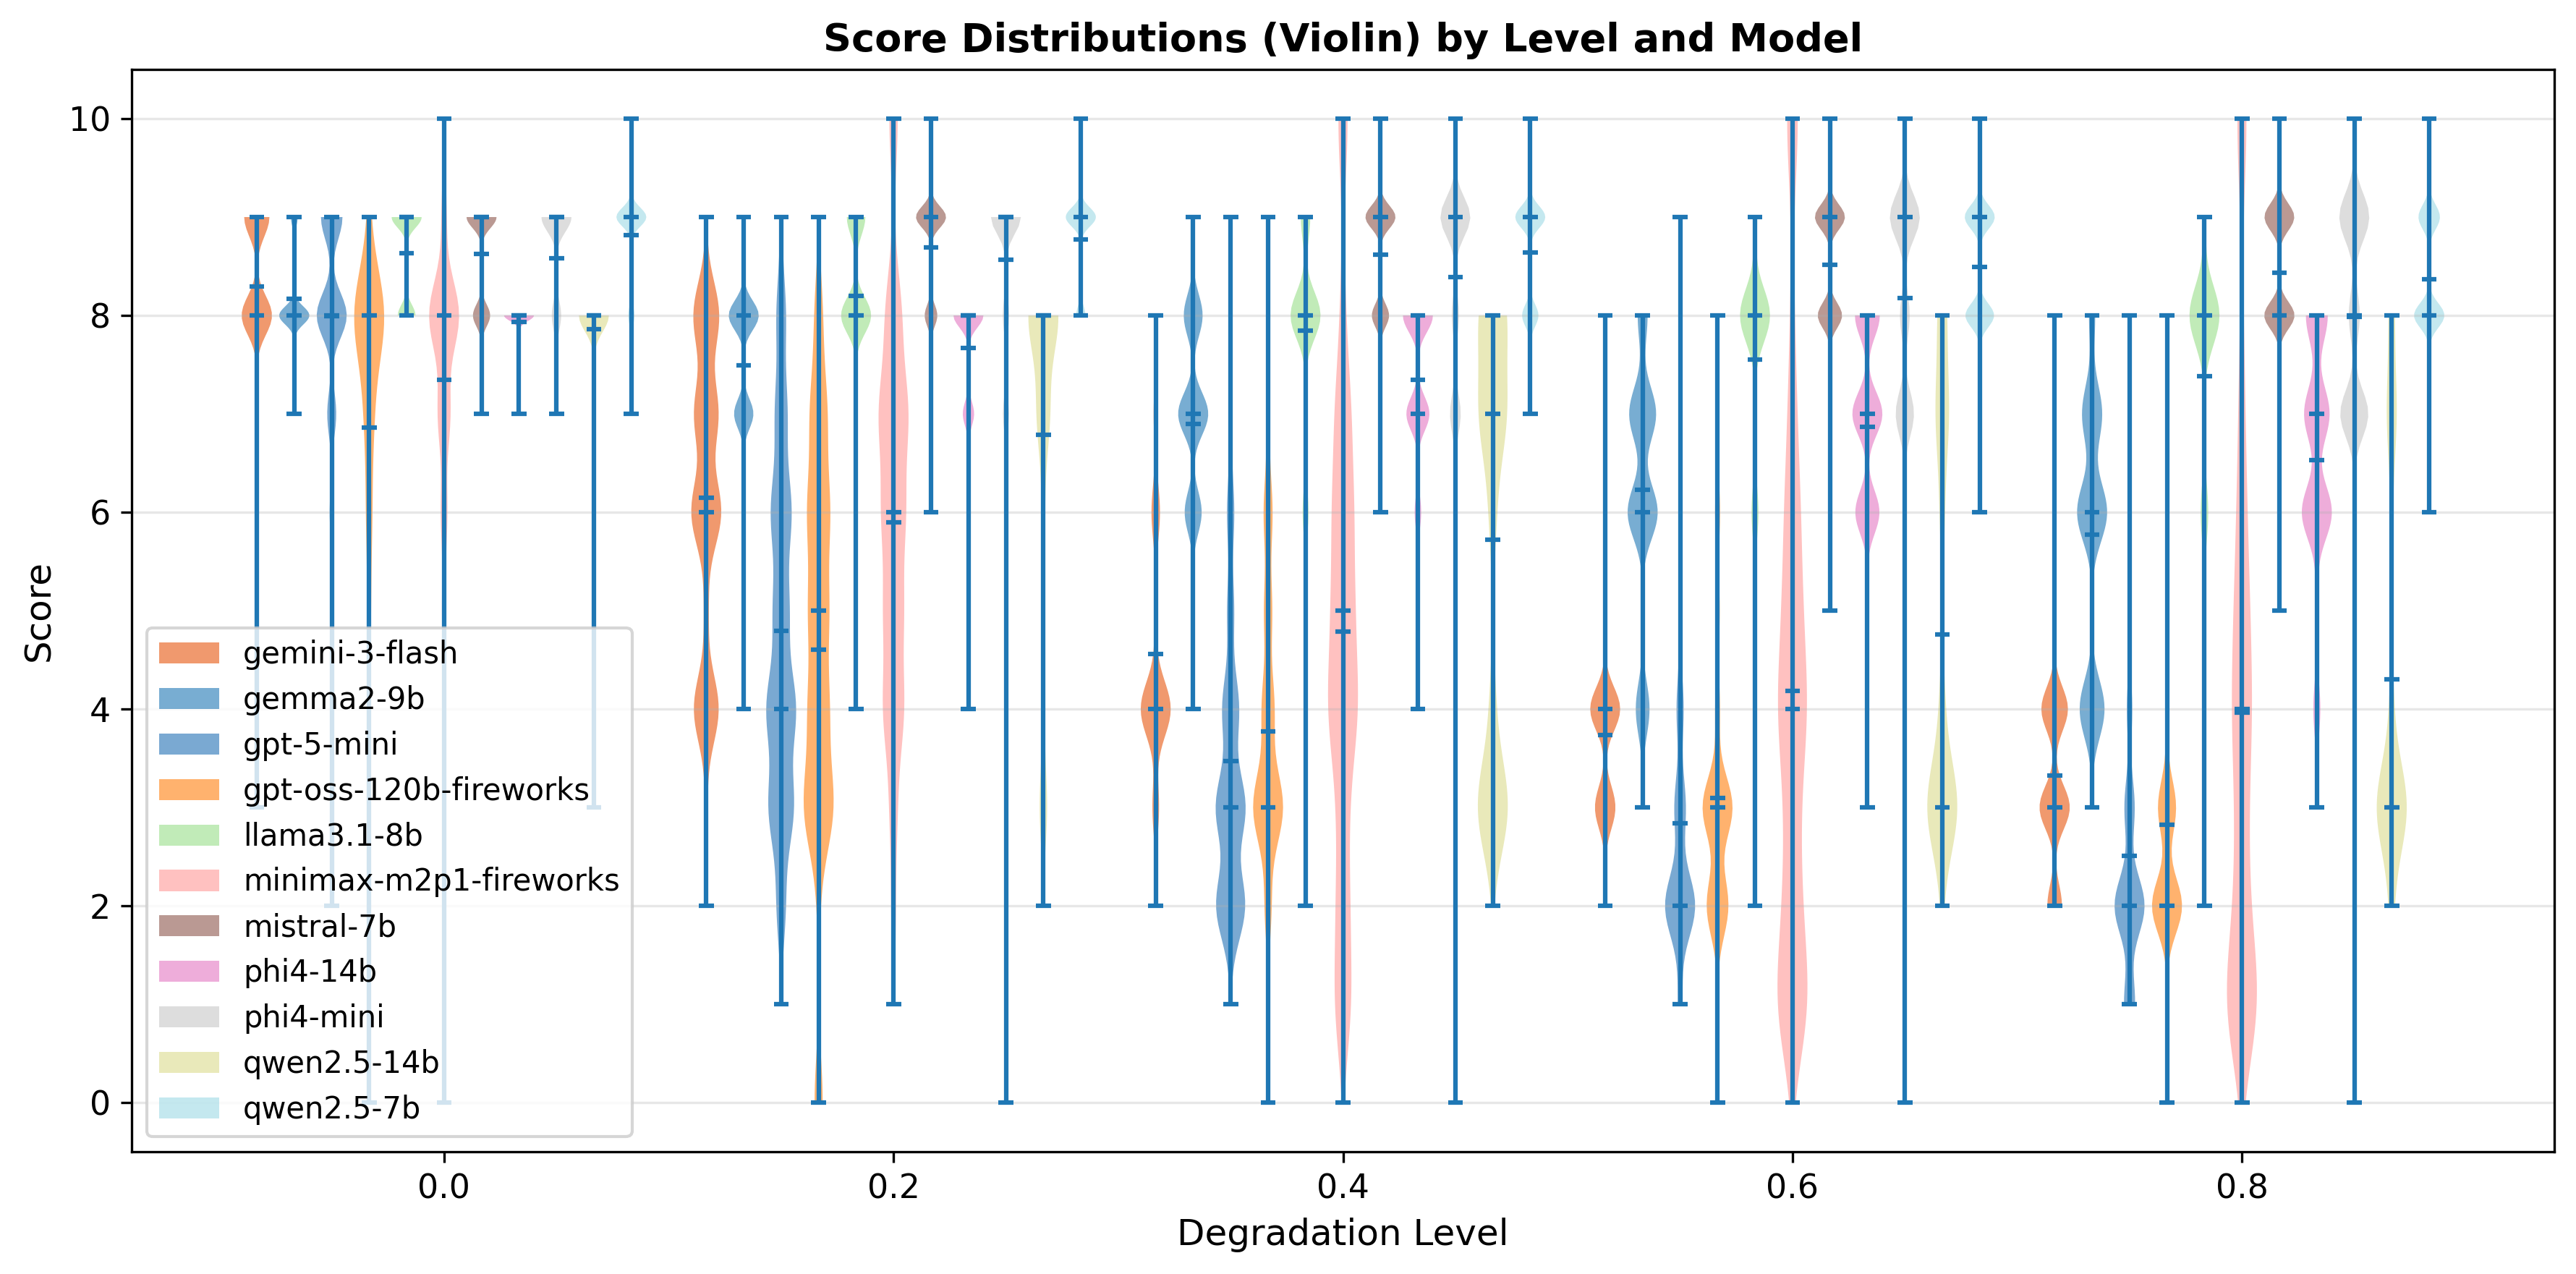
\includegraphics[width=\textwidth]{G7_violins.png}
\caption{Violin plots of score distributions by degradation level and model. The bimodal shape at $\lambda = 0.2$ reflects the mixture of high and low scores as degradation begins to take effect.}
\label{fig:violins}
\end{figure}

\end{document}
